\documentclass[11pt]{article}
\usepackage[textwidth=18.0cm, textheight=23.0cm, top=2.0cm]{geometry}
\usepackage{pst-all}
\usepackage{amssymb}
\usepackage{tikz}
\usepackage{underscore}\begin{document}
\pagestyle{empty}


ClassName: \underline{\textbf{Class_03.2bp-37}}
\par
BinSize: \underline{\textbf{40 × 40}}
\par
ReduceSize: \underline{\textbf{40 × 40}}
\par
TypeNum: \underline{\textbf{76}}
\par
Num: \underline{\textbf{80}}
\par
OutS: \underline{\textbf{35200}}
\par
InS: \underline{\textbf{28863}}
\par
Rate: \underline{\textbf{0.820}}
\par
UB: \underline{\textbf{22}}
\par
LB0: \underline{\textbf{22}}
\par
LB: \underline{\textbf{22}}
\par
LBWithCut: \underline{\textbf{22}}
\par
NodeCut: \underline{\textbf{0}}
\par
ExtendedNodeCnt: \underline{\textbf{1}}
\par
GenNodeCnt: \underline{\textbf{1}}
\par
PrimalNode: \underline{\textbf{0}}
\par
ColumnCount: \underline{\textbf{22}}
\par
TotalCutCount: \underline{\textbf{0}}
\par
RootCutCount: \underline{\textbf{0}}
\par
LPSolverCnt: \underline{\textbf{1}}
\par
PricingSolverCnt: \underline{\textbf{0}}
\par
BranchAndBoundNum: \underline{\textbf{1}}
\par
isOpt: \underline{\textbf{true}}
\par
TimeOnInitSolution: \underline{\textbf{600.000 s}}
\par
TimeOnPrimal: \underline{\textbf{0.000 s}}
\par
TimeOnPricing: \underline{\textbf{0.000 s}}
\par
TimeOnRmp: \underline{\textbf{0.078 s}}
\par
TotalTime: \underline{\textbf{600.359 s}}
\par
\newpage


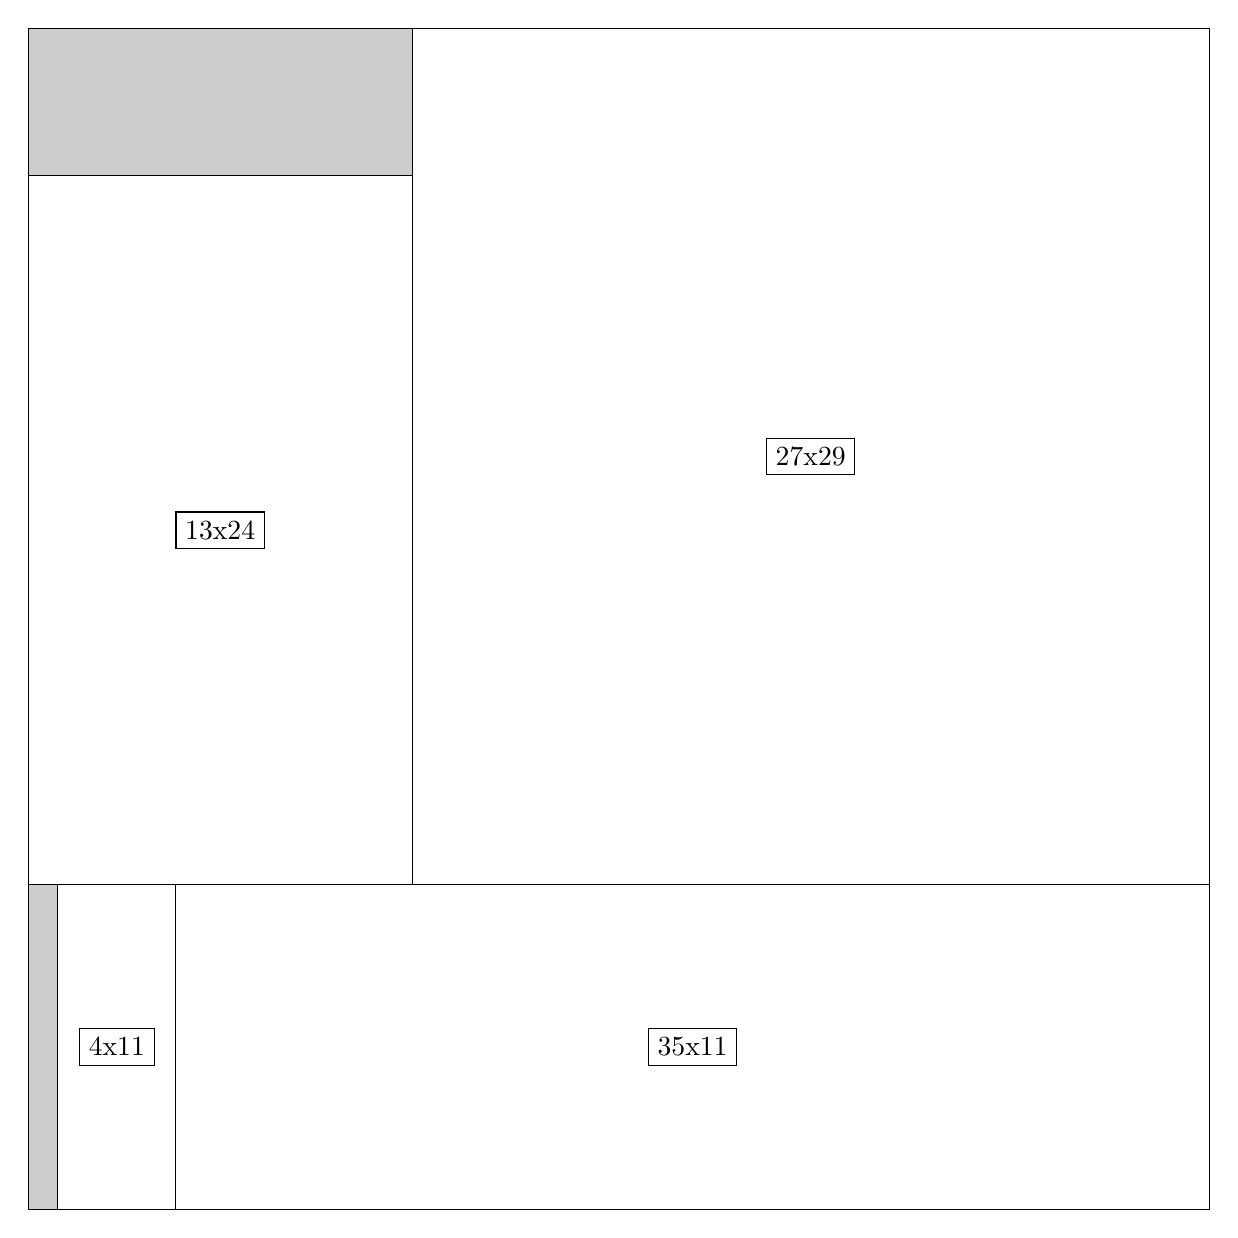
\begin{tikzpicture}[shorten >=1pt,scale=1.0,every node/.style={scale=1.0},->]
\tikzstyle{vertex}=[circle,fill=black!25,minimum size=14pt,inner sep=0pt]
\filldraw[fill=gray!40!white, draw=black] (0,0) rectangle (15.0,15.0);
\foreach \name/\x/\y/\w/\h in {35x11/1.875/0.0/13.125/4.125,4x11/0.375/0.0/1.5/4.125,27x29/4.875/4.125/10.125/10.875,13x24/0.0/4.125/4.875/9.0}
\filldraw[fill=white!40!white, draw=black] (\x,\y) rectangle node[draw] (\name) {\name} ++(\w,\h);
\end{tikzpicture}


w =35 , h =11 , x =5 , y =0 , v =385
\par
w =4 , h =11 , x =1 , y =0 , v =44
\par
w =27 , h =29 , x =13 , y =11 , v =783
\par
w =13 , h =24 , x =0 , y =11 , v =312
\par
\newpage


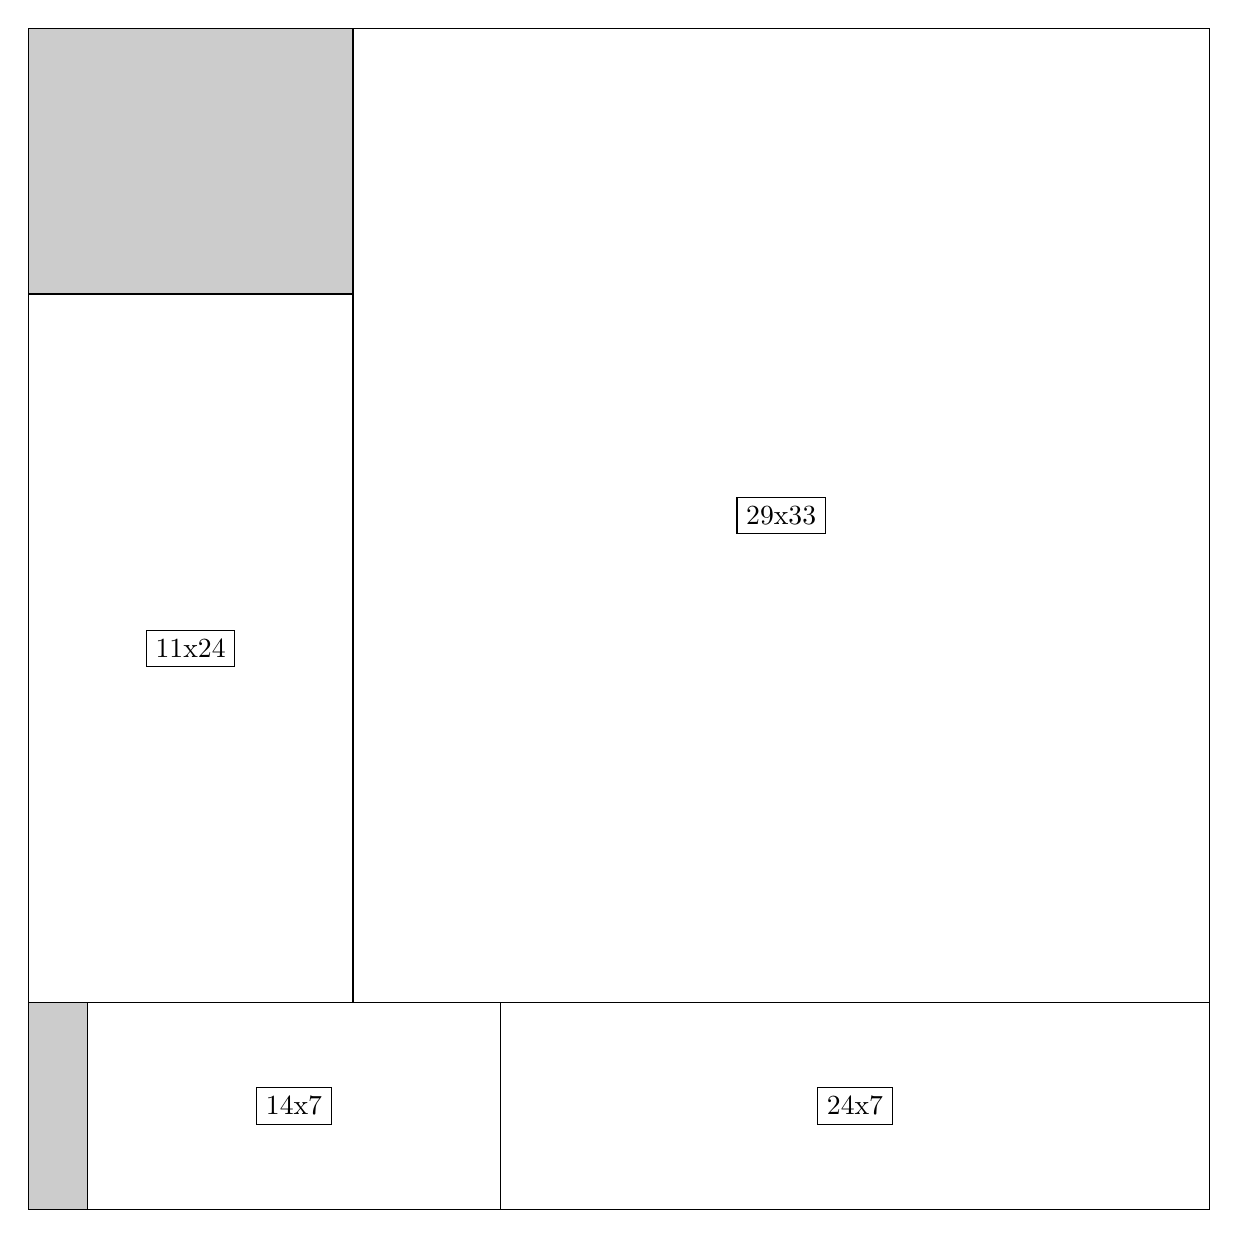
\begin{tikzpicture}[shorten >=1pt,scale=1.0,every node/.style={scale=1.0},->]
\tikzstyle{vertex}=[circle,fill=black!25,minimum size=14pt,inner sep=0pt]
\filldraw[fill=gray!40!white, draw=black] (0,0) rectangle (15.0,15.0);
\foreach \name/\x/\y/\w/\h in {24x7/6.0/0.0/9.0/2.625,14x7/0.75/0.0/5.25/2.625,29x33/4.125/2.625/10.875/12.375,11x24/0.0/2.625/4.125/9.0}
\filldraw[fill=white!40!white, draw=black] (\x,\y) rectangle node[draw] (\name) {\name} ++(\w,\h);
\end{tikzpicture}


w =24 , h =7 , x =16 , y =0 , v =168
\par
w =14 , h =7 , x =2 , y =0 , v =98
\par
w =29 , h =33 , x =11 , y =7 , v =957
\par
w =11 , h =24 , x =0 , y =7 , v =264
\par
\newpage


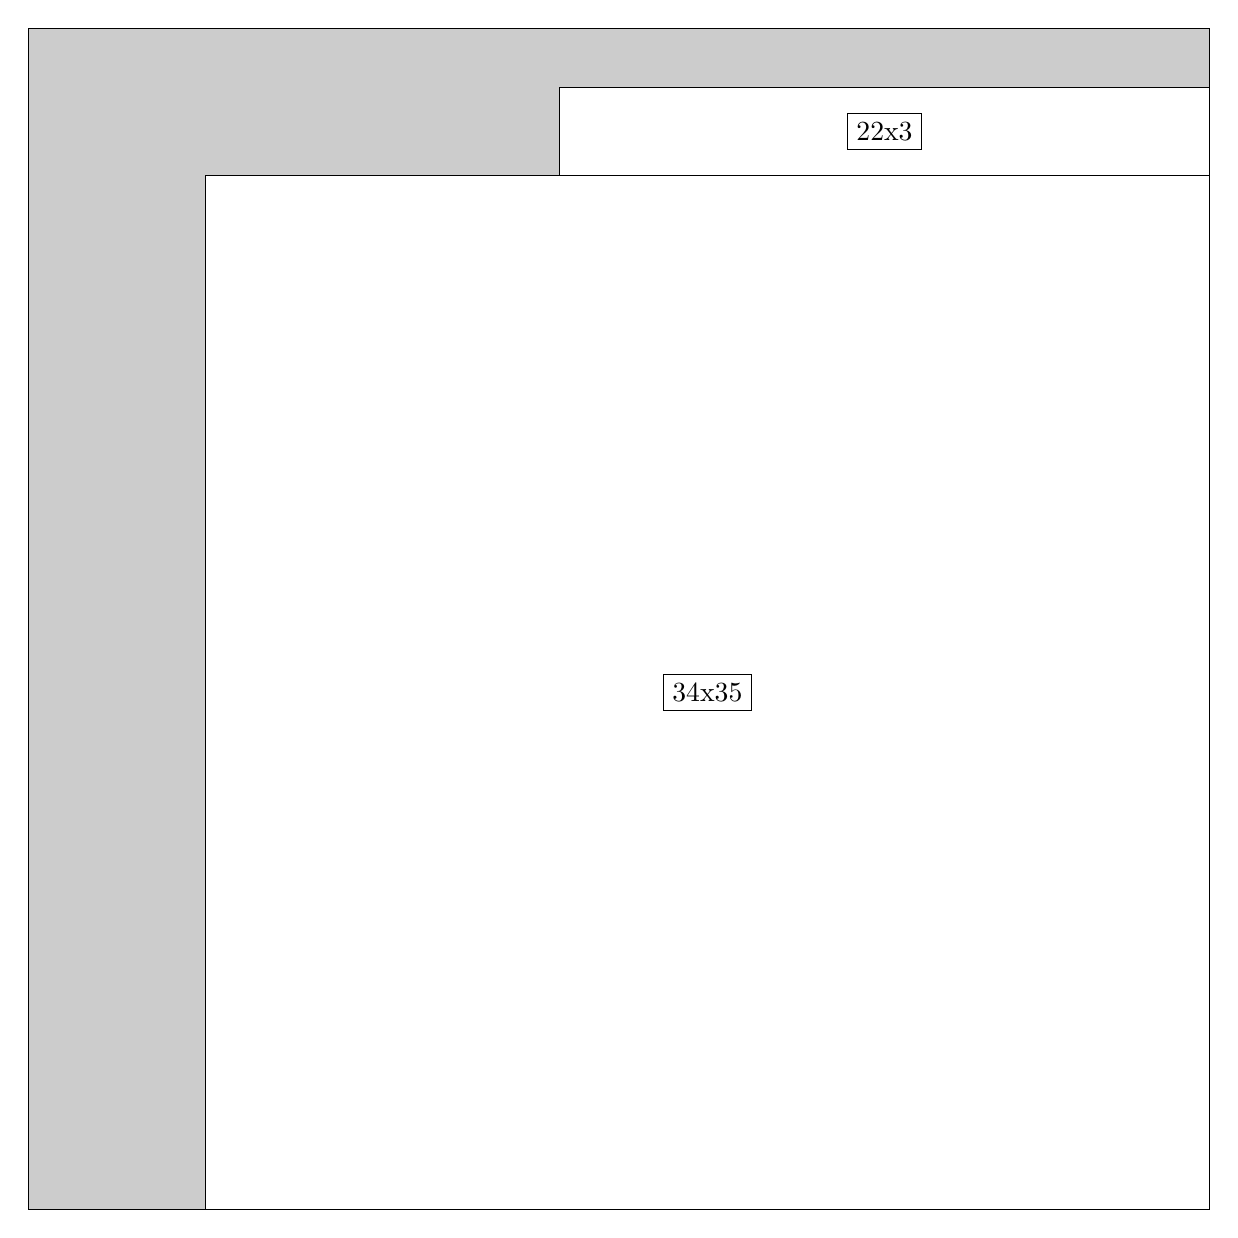
\begin{tikzpicture}[shorten >=1pt,scale=1.0,every node/.style={scale=1.0},->]
\tikzstyle{vertex}=[circle,fill=black!25,minimum size=14pt,inner sep=0pt]
\filldraw[fill=gray!40!white, draw=black] (0,0) rectangle (15.0,15.0);
\foreach \name/\x/\y/\w/\h in {34x35/2.25/0.0/12.75/13.125,22x3/6.75/13.125/8.25/1.125}
\filldraw[fill=white!40!white, draw=black] (\x,\y) rectangle node[draw] (\name) {\name} ++(\w,\h);
\end{tikzpicture}


w =34 , h =35 , x =6 , y =0 , v =1190
\par
w =22 , h =3 , x =18 , y =35 , v =66
\par
\newpage


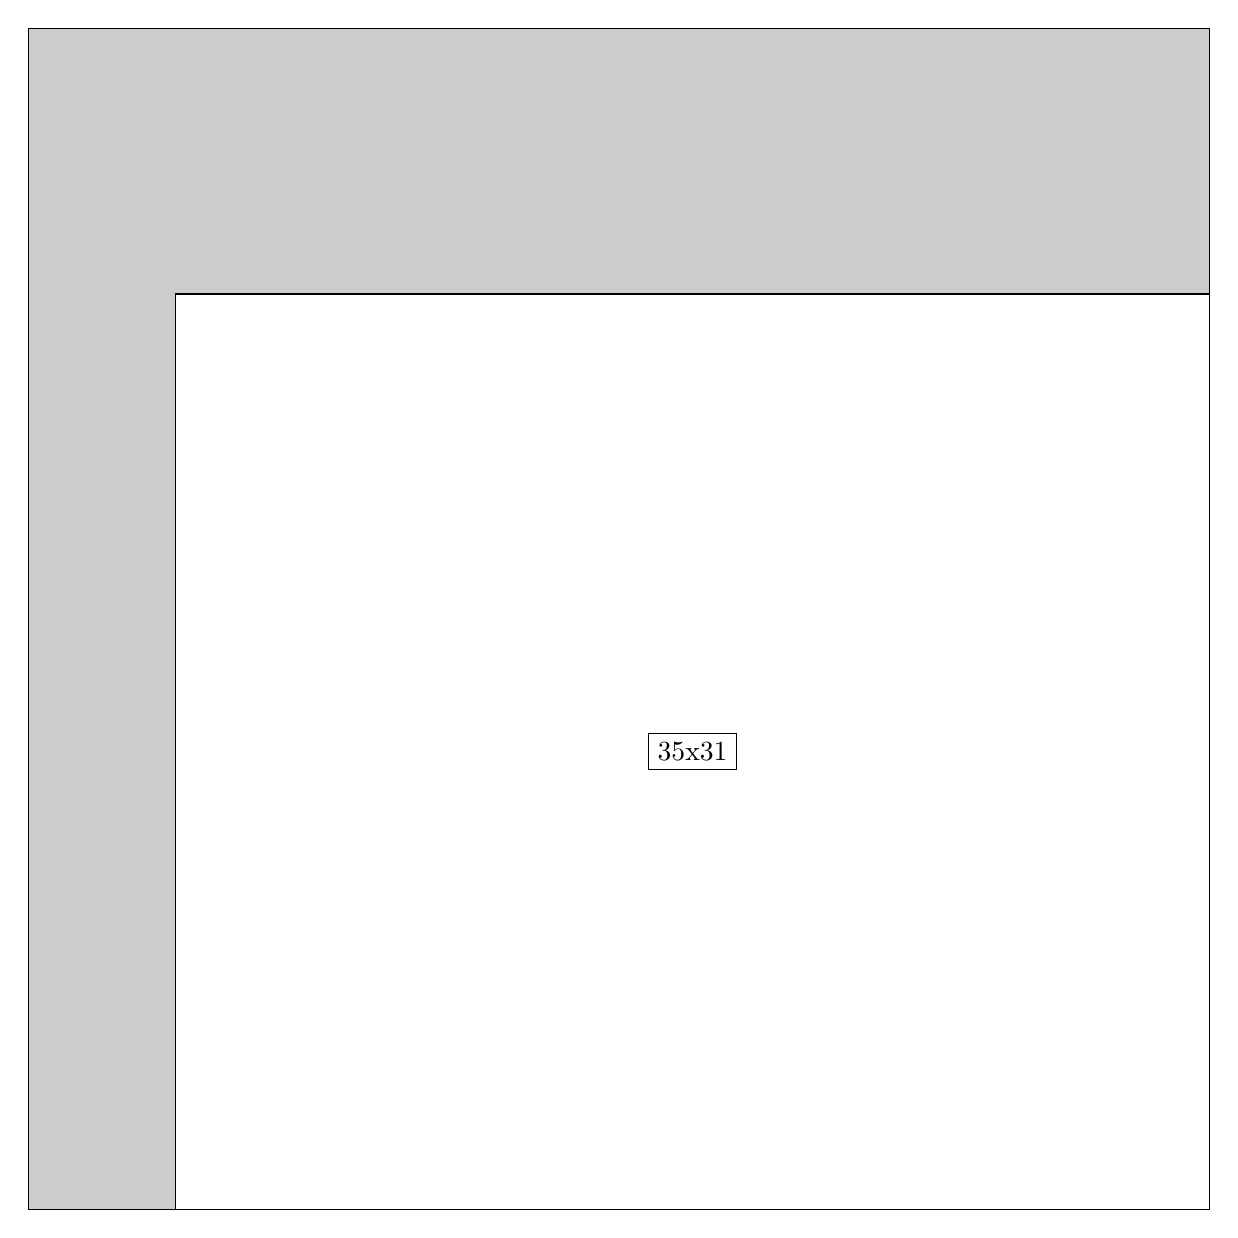
\begin{tikzpicture}[shorten >=1pt,scale=1.0,every node/.style={scale=1.0},->]
\tikzstyle{vertex}=[circle,fill=black!25,minimum size=14pt,inner sep=0pt]
\filldraw[fill=gray!40!white, draw=black] (0,0) rectangle (15.0,15.0);
\foreach \name/\x/\y/\w/\h in {35x31/1.875/0.0/13.125/11.625}
\filldraw[fill=white!40!white, draw=black] (\x,\y) rectangle node[draw] (\name) {\name} ++(\w,\h);
\end{tikzpicture}


w =35 , h =31 , x =5 , y =0 , v =1085
\par
\newpage


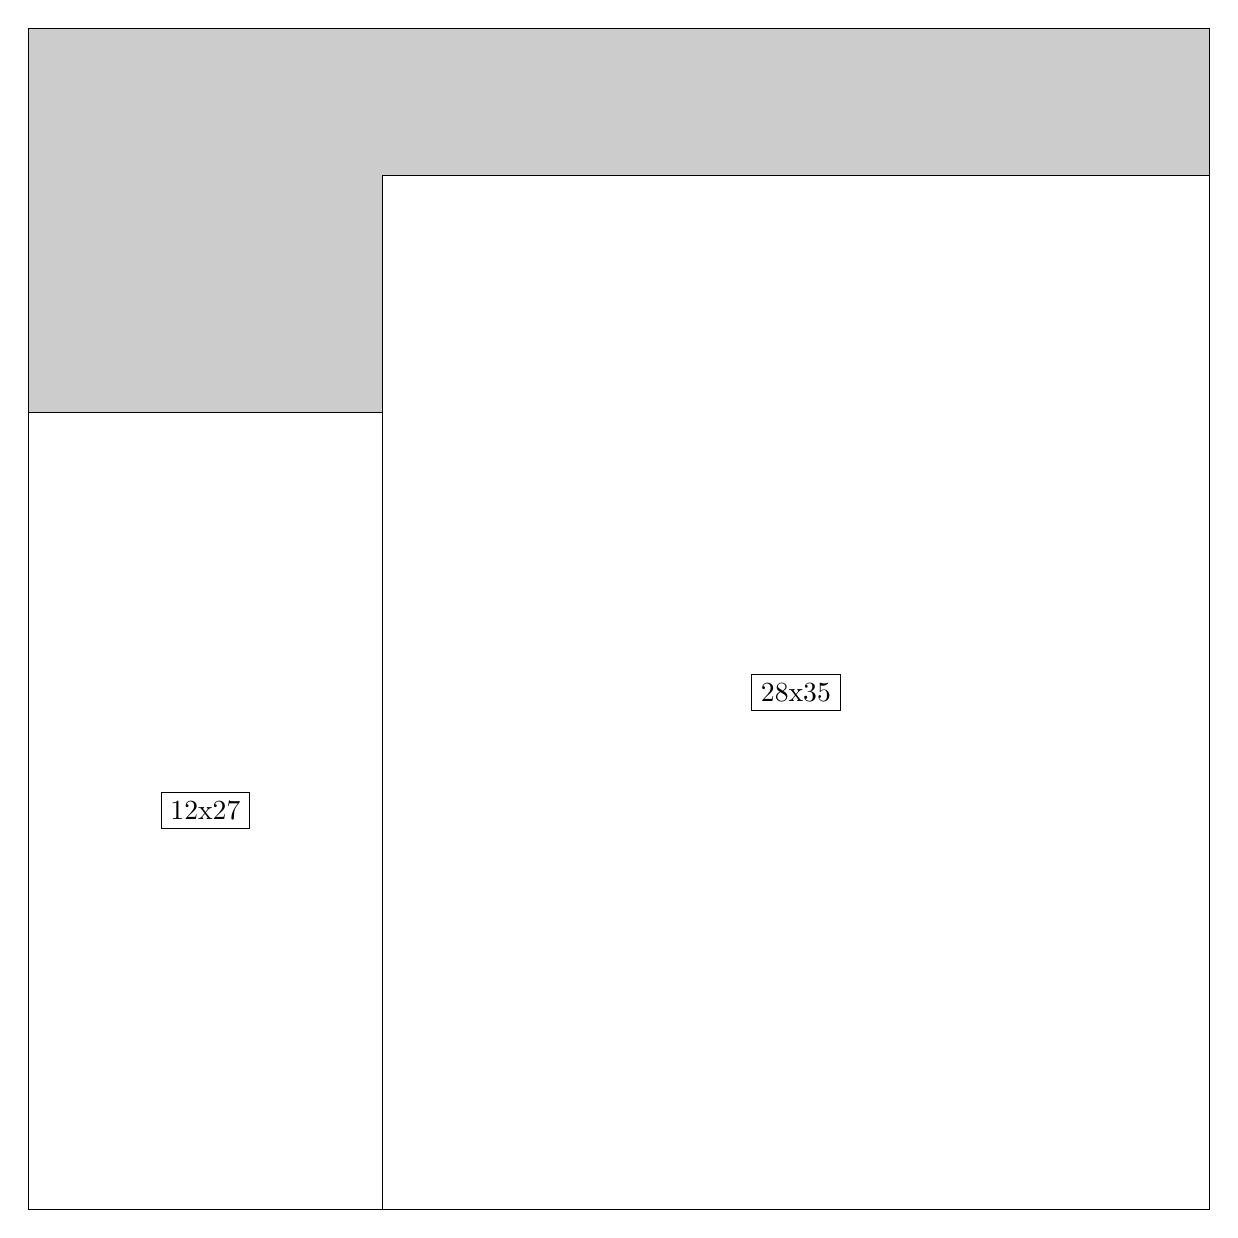
\begin{tikzpicture}[shorten >=1pt,scale=1.0,every node/.style={scale=1.0},->]
\tikzstyle{vertex}=[circle,fill=black!25,minimum size=14pt,inner sep=0pt]
\filldraw[fill=gray!40!white, draw=black] (0,0) rectangle (15.0,15.0);
\foreach \name/\x/\y/\w/\h in {28x35/4.5/0.0/10.5/13.125,12x27/0.0/0.0/4.5/10.125}
\filldraw[fill=white!40!white, draw=black] (\x,\y) rectangle node[draw] (\name) {\name} ++(\w,\h);
\end{tikzpicture}


w =28 , h =35 , x =12 , y =0 , v =980
\par
w =12 , h =27 , x =0 , y =0 , v =324
\par
\newpage


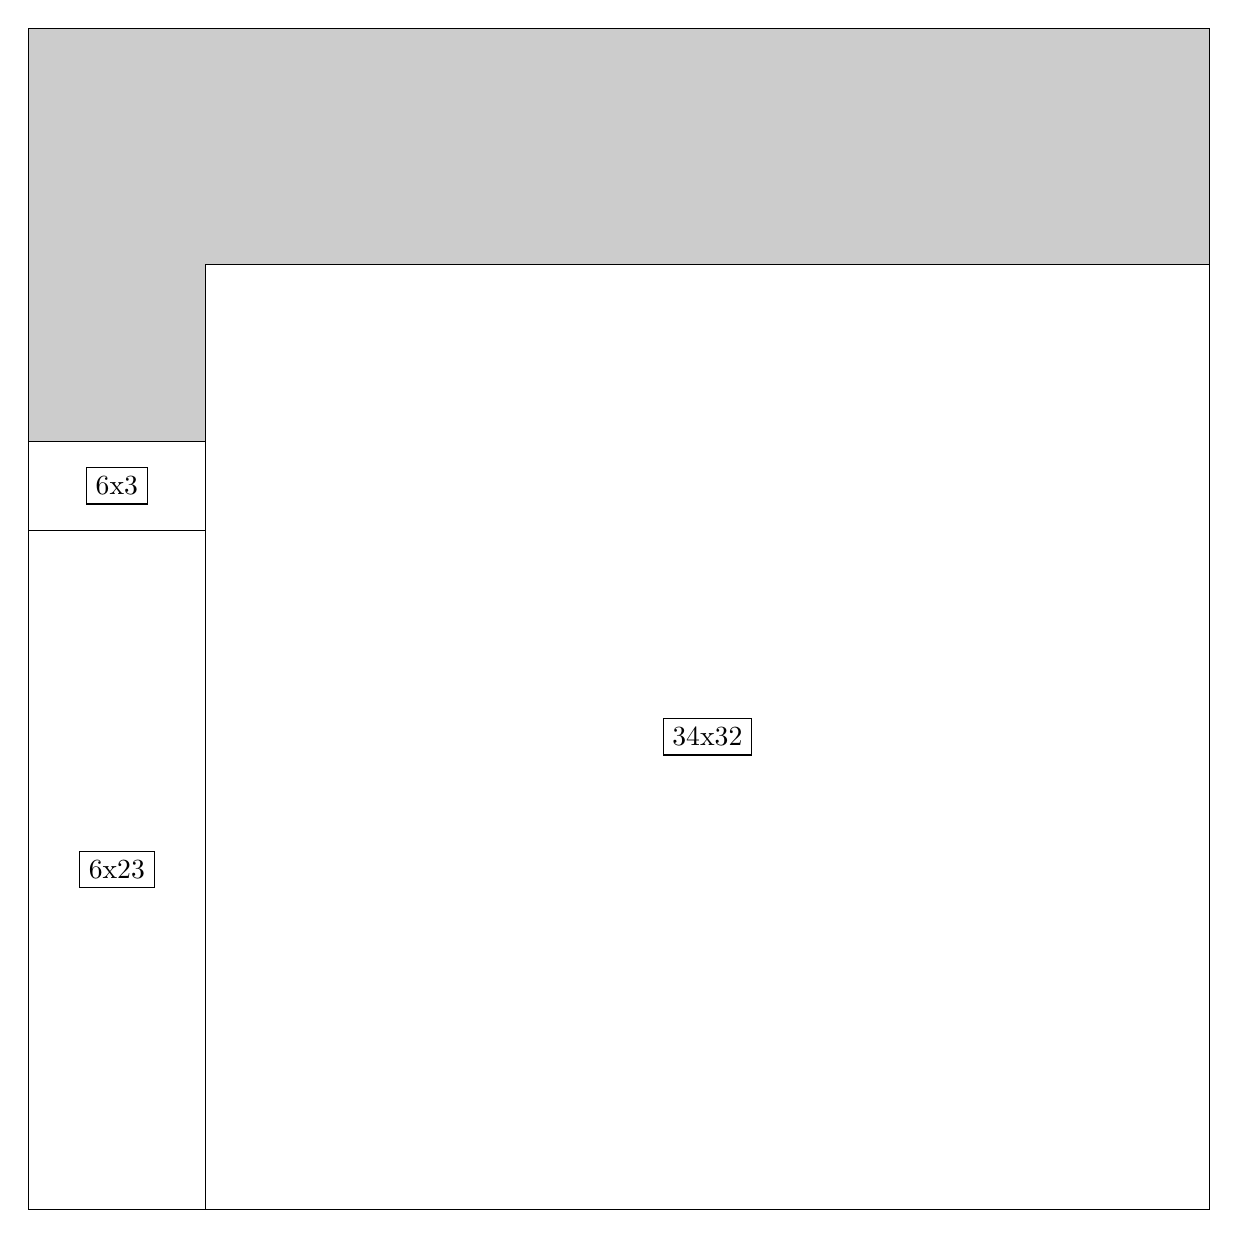
\begin{tikzpicture}[shorten >=1pt,scale=1.0,every node/.style={scale=1.0},->]
\tikzstyle{vertex}=[circle,fill=black!25,minimum size=14pt,inner sep=0pt]
\filldraw[fill=gray!40!white, draw=black] (0,0) rectangle (15.0,15.0);
\foreach \name/\x/\y/\w/\h in {34x32/2.25/0.0/12.75/12.0,6x23/0.0/0.0/2.25/8.625,6x3/0.0/8.625/2.25/1.125}
\filldraw[fill=white!40!white, draw=black] (\x,\y) rectangle node[draw] (\name) {\name} ++(\w,\h);
\end{tikzpicture}


w =34 , h =32 , x =6 , y =0 , v =1088
\par
w =6 , h =23 , x =0 , y =0 , v =138
\par
w =6 , h =3 , x =0 , y =23 , v =18
\par
\newpage


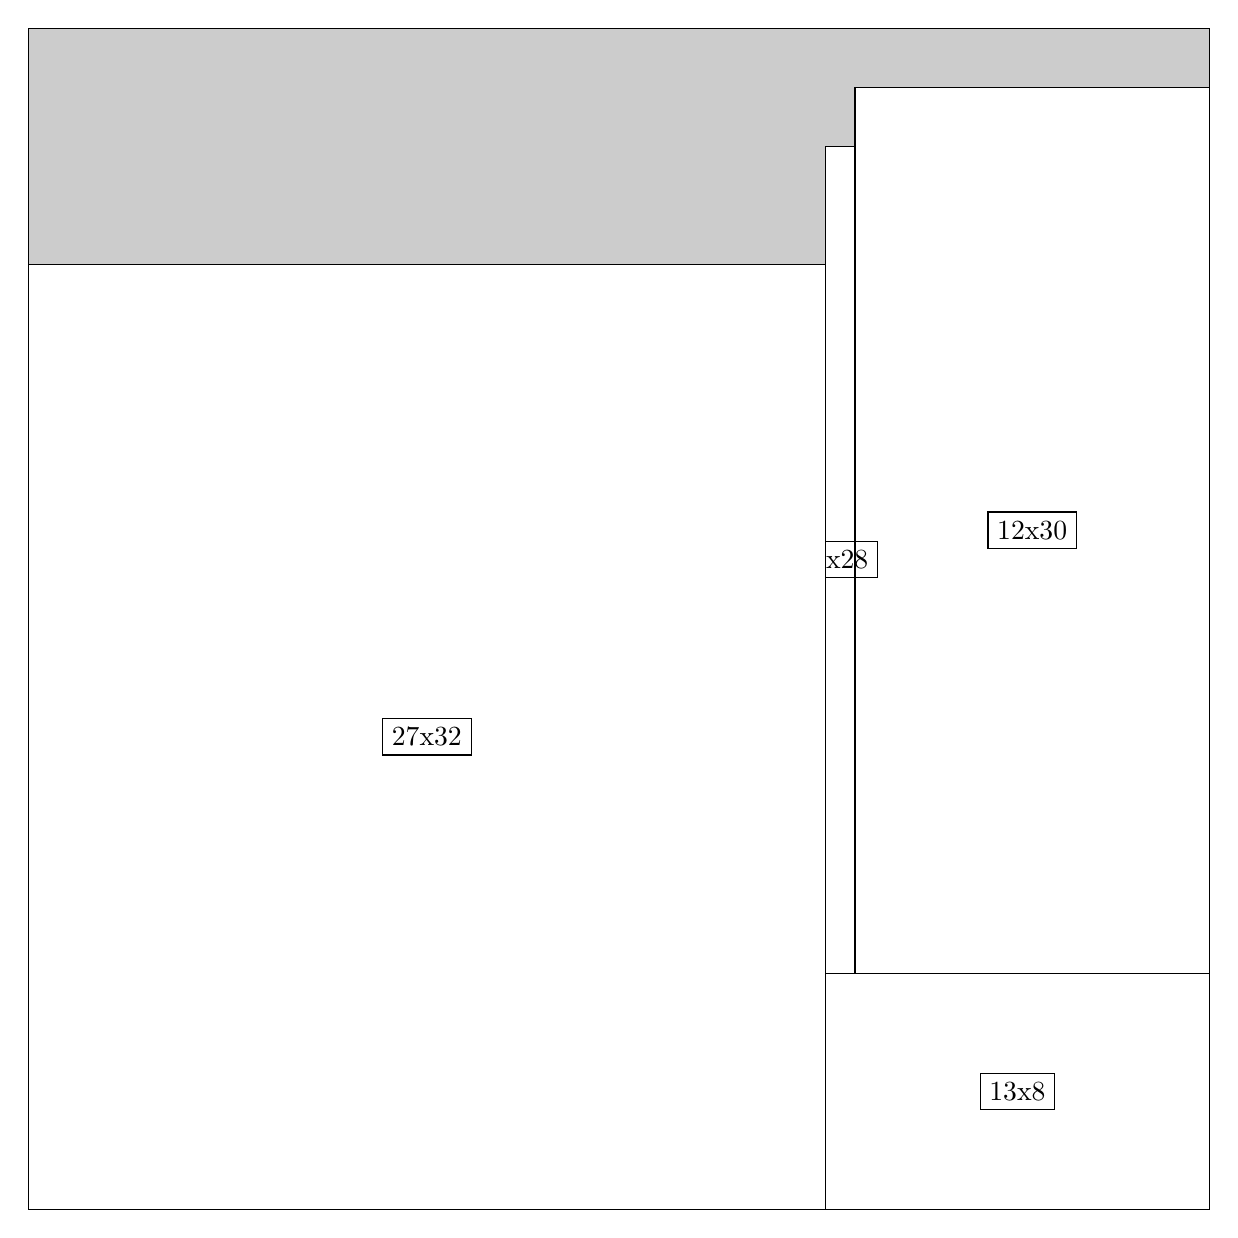
\begin{tikzpicture}[shorten >=1pt,scale=1.0,every node/.style={scale=1.0},->]
\tikzstyle{vertex}=[circle,fill=black!25,minimum size=14pt,inner sep=0pt]
\filldraw[fill=gray!40!white, draw=black] (0,0) rectangle (15.0,15.0);
\foreach \name/\x/\y/\w/\h in {13x8/10.125/0.0/4.875/3.0,12x30/10.5/3.0/4.5/11.25,1x28/10.125/3.0/0.375/10.5,27x32/0.0/0.0/10.125/12.0}
\filldraw[fill=white!40!white, draw=black] (\x,\y) rectangle node[draw] (\name) {\name} ++(\w,\h);
\end{tikzpicture}


w =13 , h =8 , x =27 , y =0 , v =104
\par
w =12 , h =30 , x =28 , y =8 , v =360
\par
w =1 , h =28 , x =27 , y =8 , v =28
\par
w =27 , h =32 , x =0 , y =0 , v =864
\par
\newpage


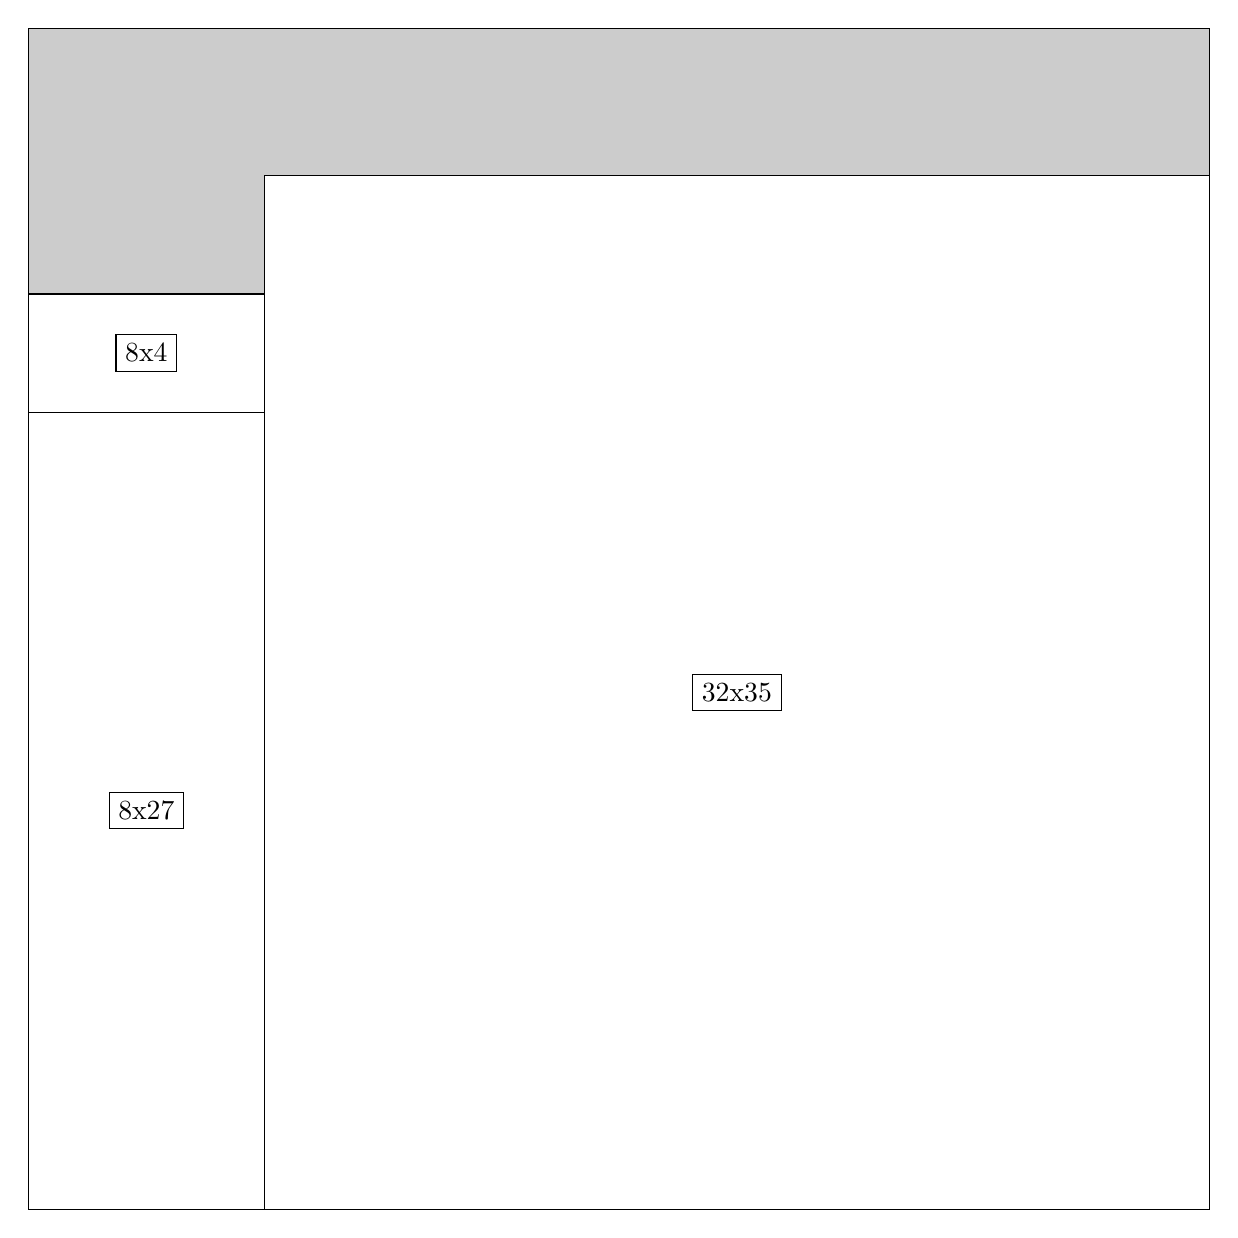
\begin{tikzpicture}[shorten >=1pt,scale=1.0,every node/.style={scale=1.0},->]
\tikzstyle{vertex}=[circle,fill=black!25,minimum size=14pt,inner sep=0pt]
\filldraw[fill=gray!40!white, draw=black] (0,0) rectangle (15.0,15.0);
\foreach \name/\x/\y/\w/\h in {32x35/3.0/0.0/12.0/13.125,8x27/0.0/0.0/3.0/10.125,8x4/0.0/10.125/3.0/1.5}
\filldraw[fill=white!40!white, draw=black] (\x,\y) rectangle node[draw] (\name) {\name} ++(\w,\h);
\end{tikzpicture}


w =32 , h =35 , x =8 , y =0 , v =1120
\par
w =8 , h =27 , x =0 , y =0 , v =216
\par
w =8 , h =4 , x =0 , y =27 , v =32
\par
\newpage


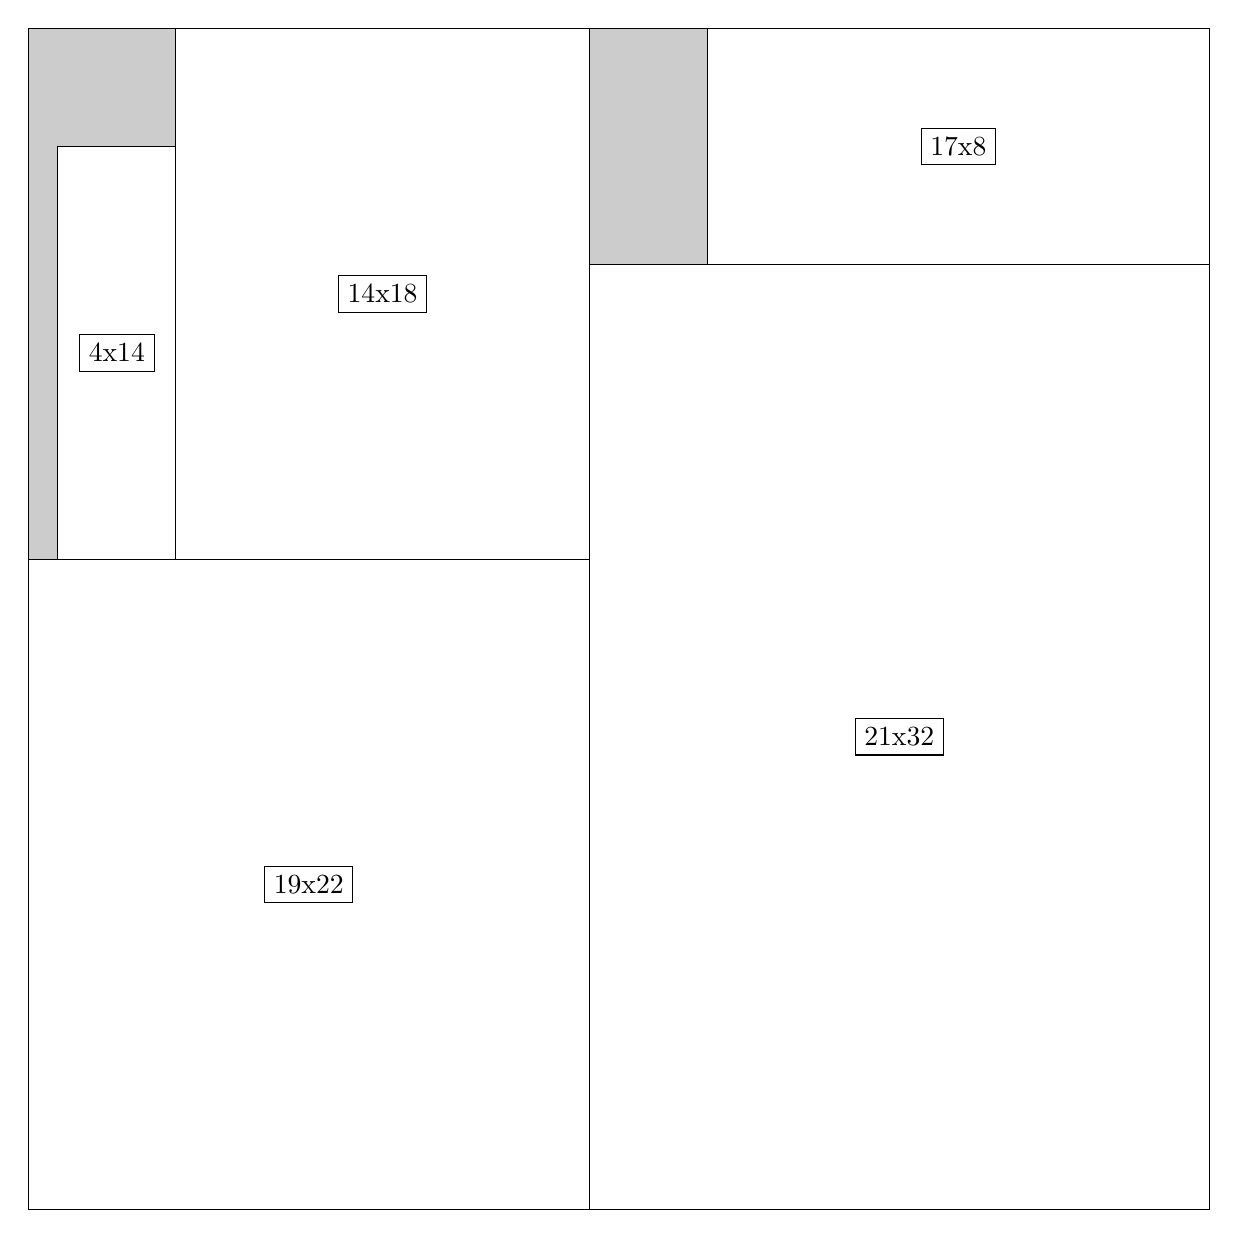
\begin{tikzpicture}[shorten >=1pt,scale=1.0,every node/.style={scale=1.0},->]
\tikzstyle{vertex}=[circle,fill=black!25,minimum size=14pt,inner sep=0pt]
\filldraw[fill=gray!40!white, draw=black] (0,0) rectangle (15.0,15.0);
\foreach \name/\x/\y/\w/\h in {21x32/7.125/0.0/7.875/12.0,17x8/8.625/12.0/6.375/3.0,19x22/0.0/0.0/7.125/8.25,14x18/1.875/8.25/5.25/6.75,4x14/0.375/8.25/1.5/5.25}
\filldraw[fill=white!40!white, draw=black] (\x,\y) rectangle node[draw] (\name) {\name} ++(\w,\h);
\end{tikzpicture}


w =21 , h =32 , x =19 , y =0 , v =672
\par
w =17 , h =8 , x =23 , y =32 , v =136
\par
w =19 , h =22 , x =0 , y =0 , v =418
\par
w =14 , h =18 , x =5 , y =22 , v =252
\par
w =4 , h =14 , x =1 , y =22 , v =56
\par
\newpage


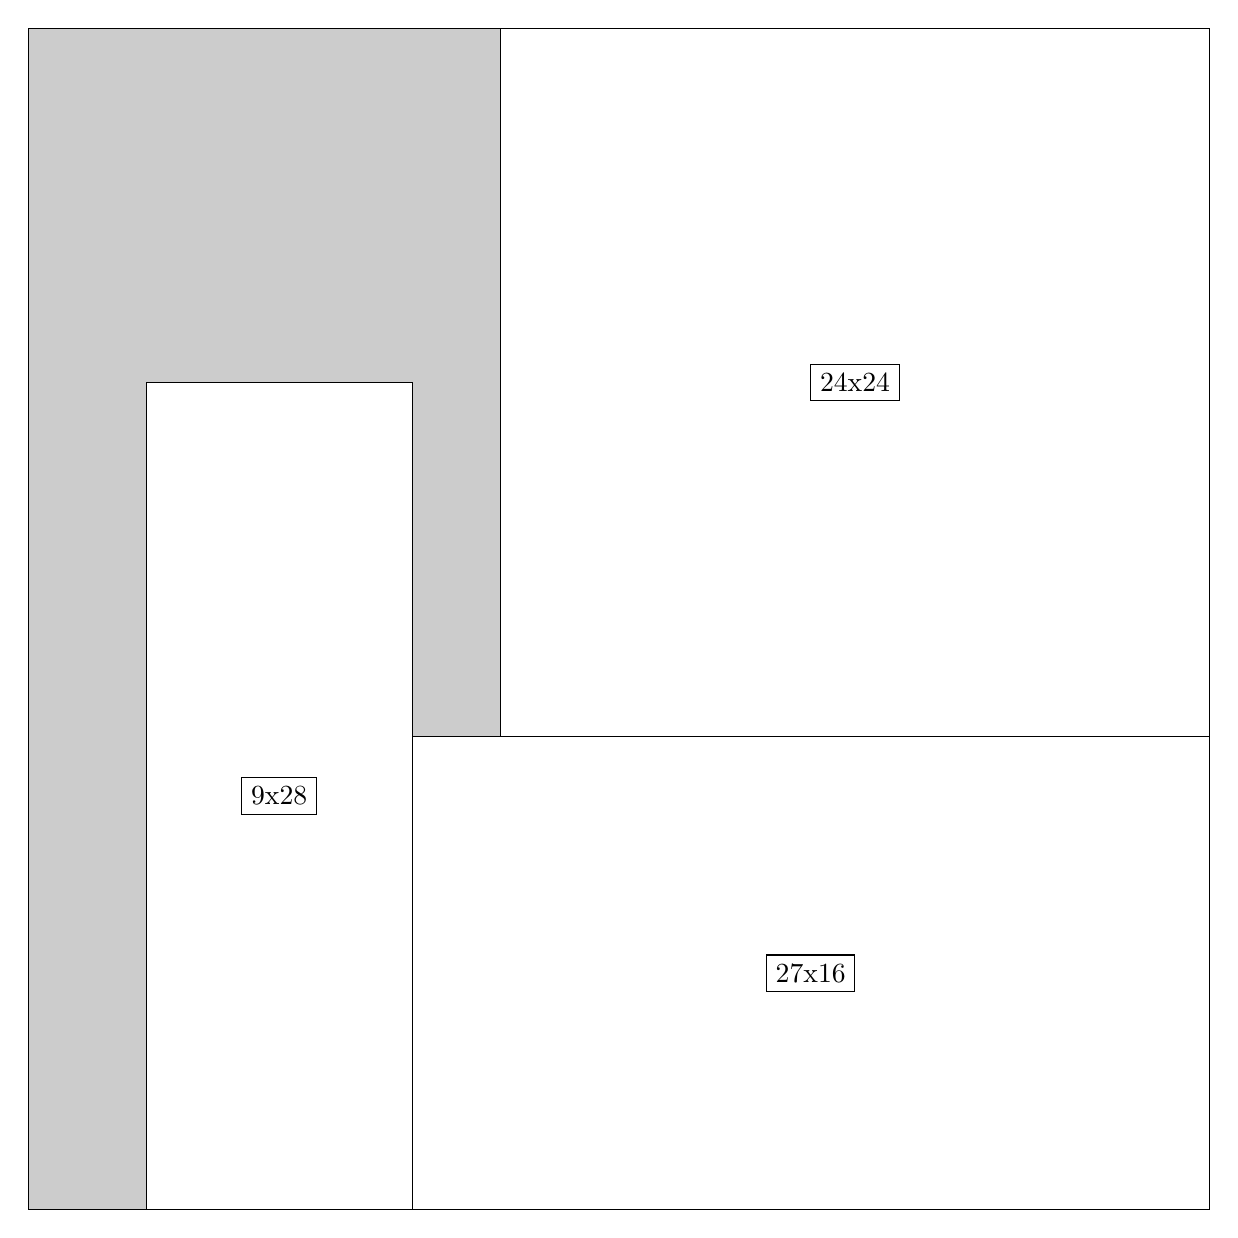
\begin{tikzpicture}[shorten >=1pt,scale=1.0,every node/.style={scale=1.0},->]
\tikzstyle{vertex}=[circle,fill=black!25,minimum size=14pt,inner sep=0pt]
\filldraw[fill=gray!40!white, draw=black] (0,0) rectangle (15.0,15.0);
\foreach \name/\x/\y/\w/\h in {27x16/4.875/0.0/10.125/6.0,24x24/6.0/6.0/9.0/9.0,9x28/1.5/0.0/3.375/10.5}
\filldraw[fill=white!40!white, draw=black] (\x,\y) rectangle node[draw] (\name) {\name} ++(\w,\h);
\end{tikzpicture}


w =27 , h =16 , x =13 , y =0 , v =432
\par
w =24 , h =24 , x =16 , y =16 , v =576
\par
w =9 , h =28 , x =4 , y =0 , v =252
\par
\newpage


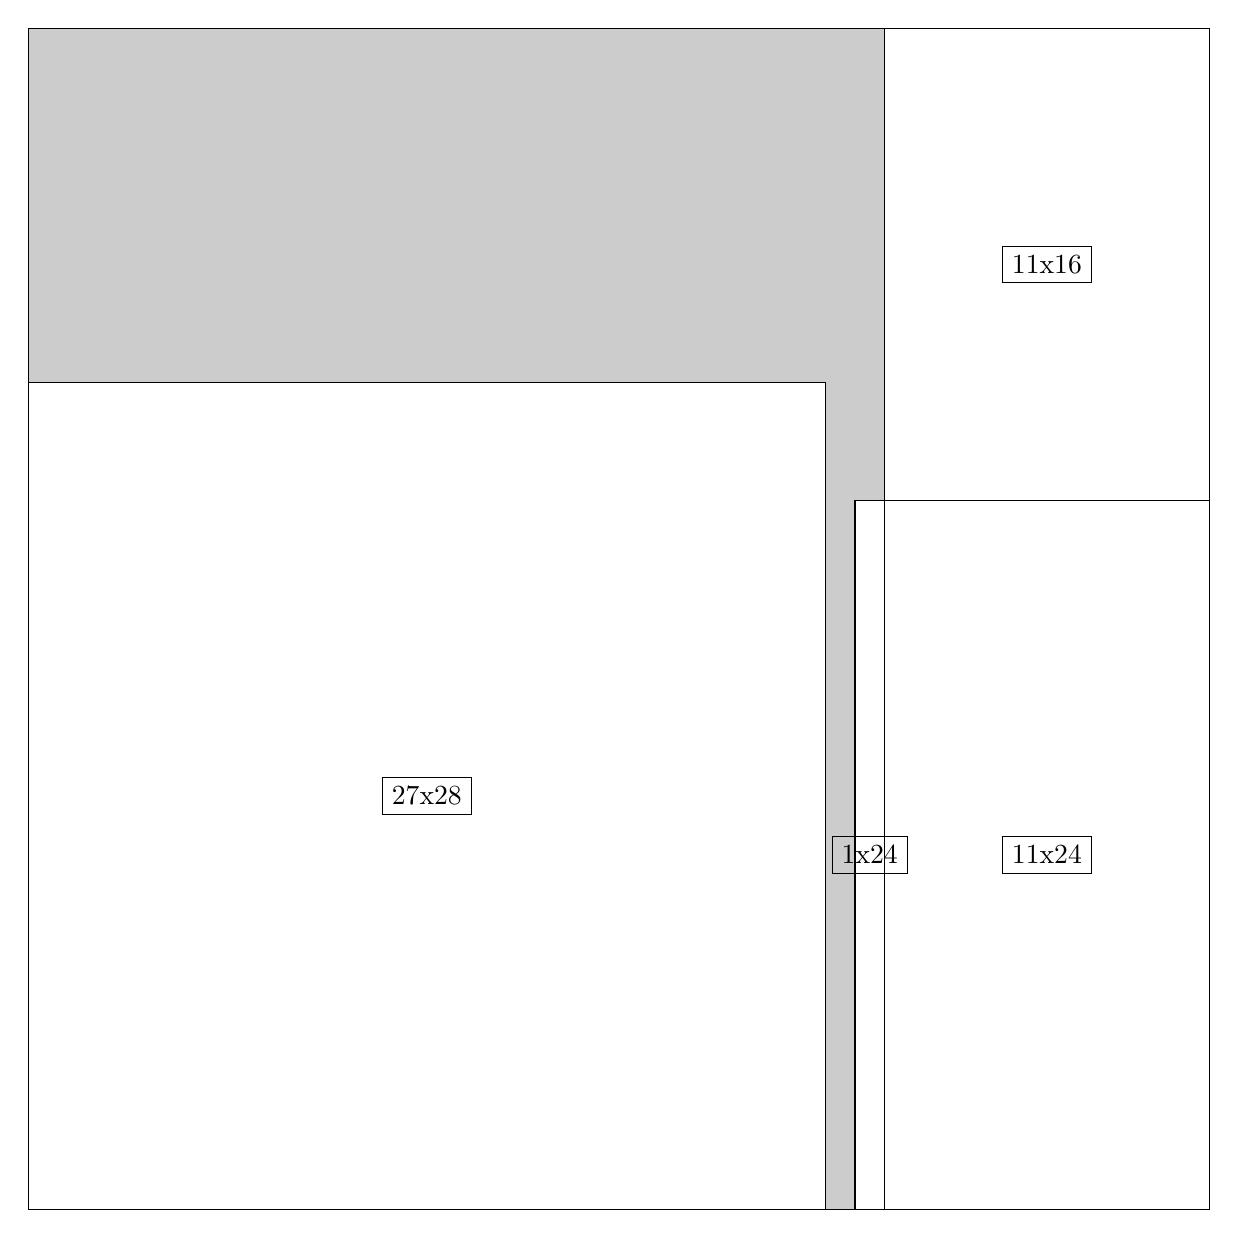
\begin{tikzpicture}[shorten >=1pt,scale=1.0,every node/.style={scale=1.0},->]
\tikzstyle{vertex}=[circle,fill=black!25,minimum size=14pt,inner sep=0pt]
\filldraw[fill=gray!40!white, draw=black] (0,0) rectangle (15.0,15.0);
\foreach \name/\x/\y/\w/\h in {11x24/10.875/0.0/4.125/9.0,1x24/10.5/0.0/0.375/9.0,11x16/10.875/9.0/4.125/6.0,27x28/0.0/0.0/10.125/10.5}
\filldraw[fill=white!40!white, draw=black] (\x,\y) rectangle node[draw] (\name) {\name} ++(\w,\h);
\end{tikzpicture}


w =11 , h =24 , x =29 , y =0 , v =264
\par
w =1 , h =24 , x =28 , y =0 , v =24
\par
w =11 , h =16 , x =29 , y =24 , v =176
\par
w =27 , h =28 , x =0 , y =0 , v =756
\par
\newpage


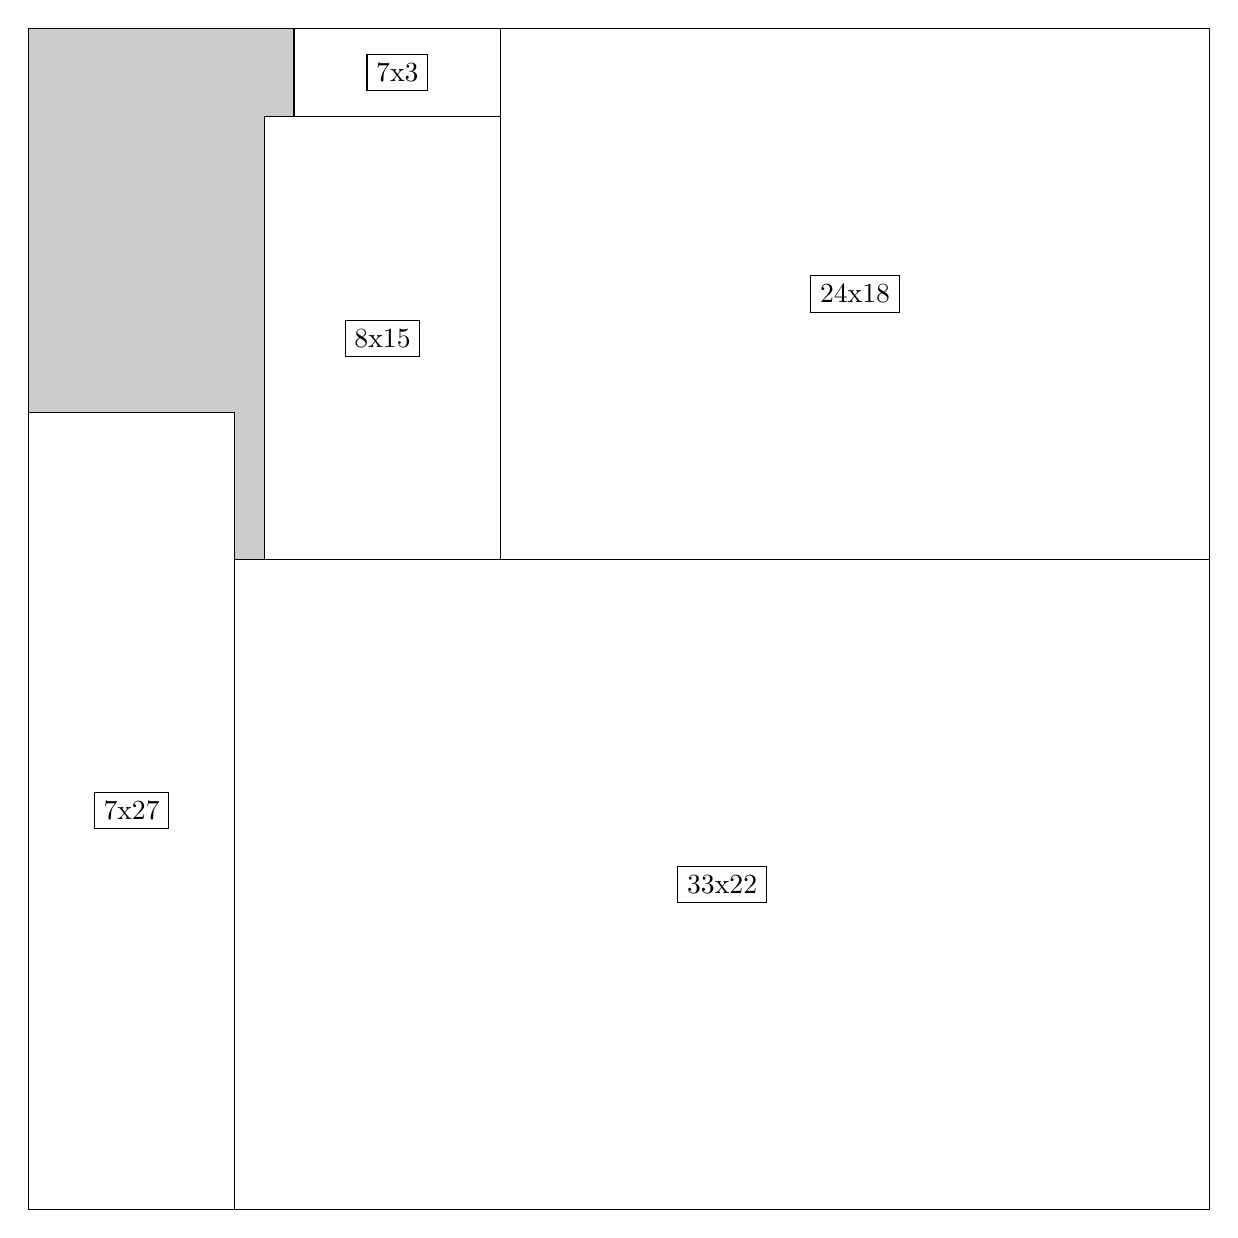
\begin{tikzpicture}[shorten >=1pt,scale=1.0,every node/.style={scale=1.0},->]
\tikzstyle{vertex}=[circle,fill=black!25,minimum size=14pt,inner sep=0pt]
\filldraw[fill=gray!40!white, draw=black] (0,0) rectangle (15.0,15.0);
\foreach \name/\x/\y/\w/\h in {33x22/2.625/0.0/12.375/8.25,24x18/6.0/8.25/9.0/6.75,8x15/3.0/8.25/3.0/5.625,7x3/3.375/13.875/2.625/1.125,7x27/0.0/0.0/2.625/10.125}
\filldraw[fill=white!40!white, draw=black] (\x,\y) rectangle node[draw] (\name) {\name} ++(\w,\h);
\end{tikzpicture}


w =33 , h =22 , x =7 , y =0 , v =726
\par
w =24 , h =18 , x =16 , y =22 , v =432
\par
w =8 , h =15 , x =8 , y =22 , v =120
\par
w =7 , h =3 , x =9 , y =37 , v =21
\par
w =7 , h =27 , x =0 , y =0 , v =189
\par
\newpage


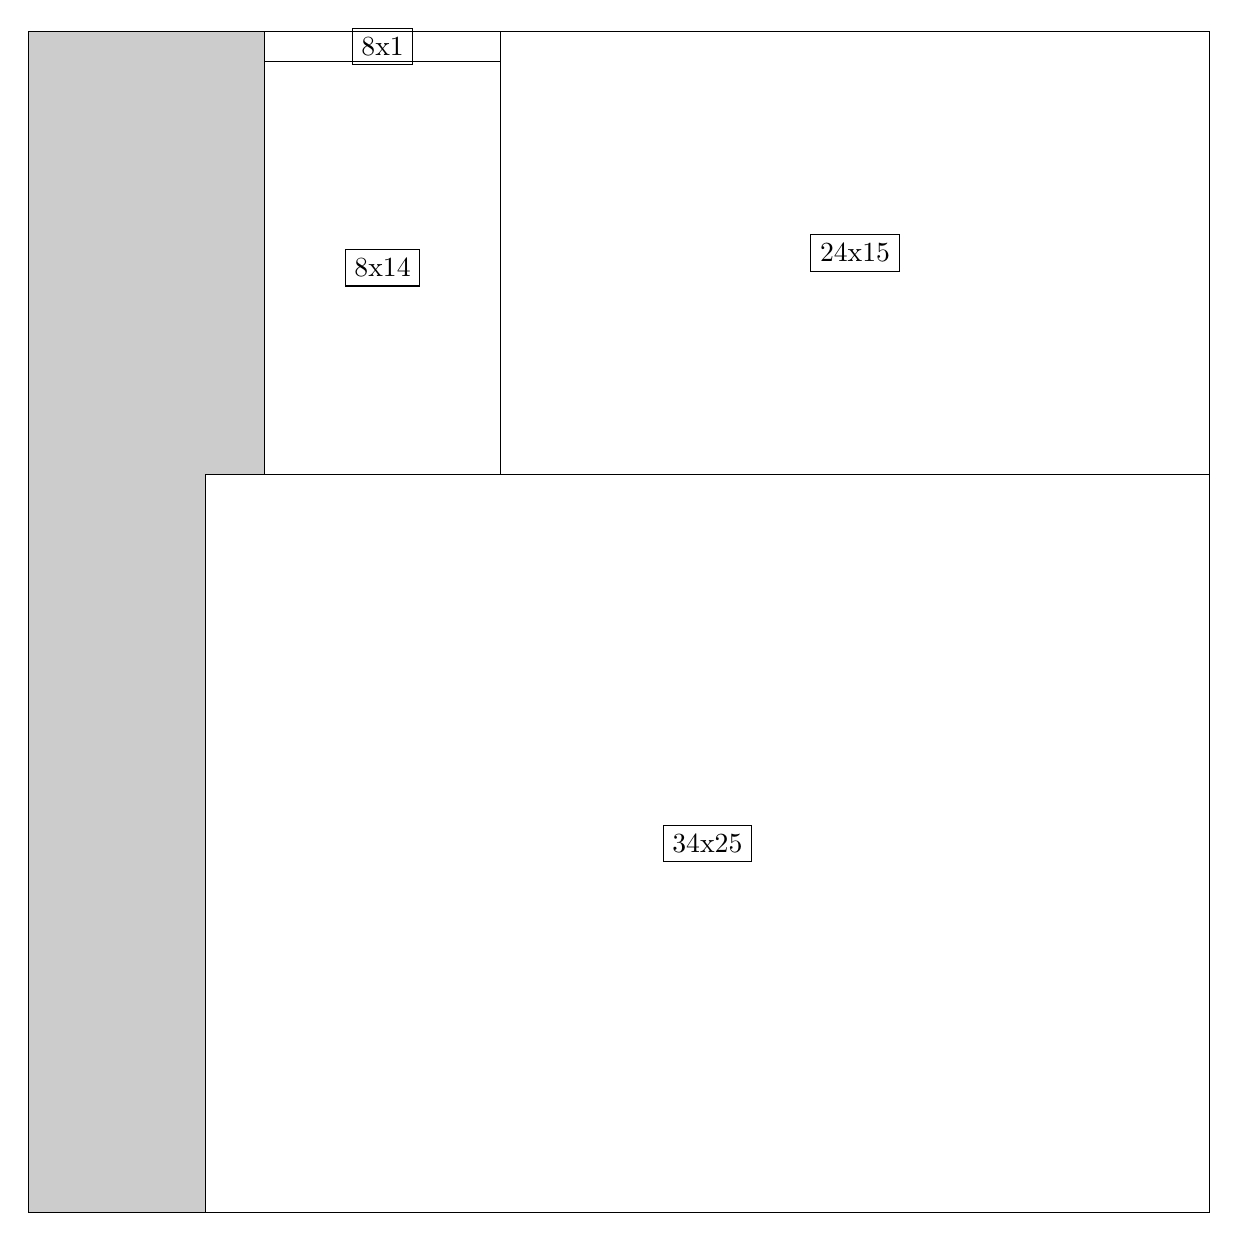
\begin{tikzpicture}[shorten >=1pt,scale=1.0,every node/.style={scale=1.0},->]
\tikzstyle{vertex}=[circle,fill=black!25,minimum size=14pt,inner sep=0pt]
\filldraw[fill=gray!40!white, draw=black] (0,0) rectangle (15.0,15.0);
\foreach \name/\x/\y/\w/\h in {34x25/2.25/0.0/12.75/9.375,24x15/6.0/9.375/9.0/5.625,8x14/3.0/9.375/3.0/5.25,8x1/3.0/14.625/3.0/0.375}
\filldraw[fill=white!40!white, draw=black] (\x,\y) rectangle node[draw] (\name) {\name} ++(\w,\h);
\end{tikzpicture}


w =34 , h =25 , x =6 , y =0 , v =850
\par
w =24 , h =15 , x =16 , y =25 , v =360
\par
w =8 , h =14 , x =8 , y =25 , v =112
\par
w =8 , h =1 , x =8 , y =39 , v =8
\par
\newpage


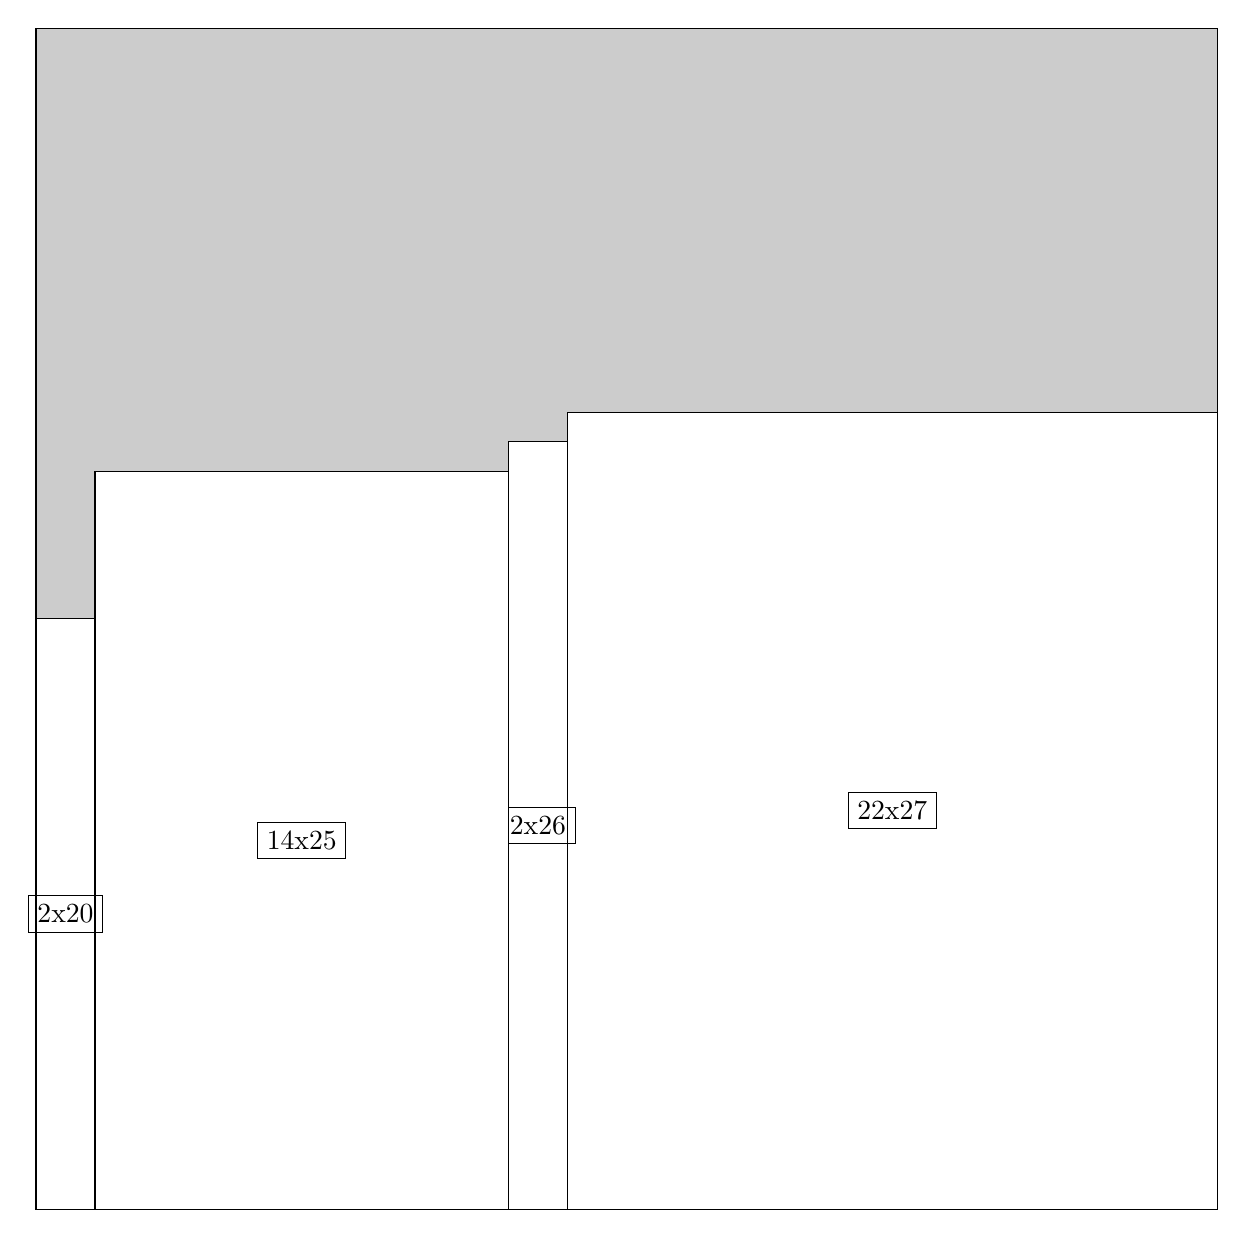
\begin{tikzpicture}[shorten >=1pt,scale=1.0,every node/.style={scale=1.0},->]
\tikzstyle{vertex}=[circle,fill=black!25,minimum size=14pt,inner sep=0pt]
\filldraw[fill=gray!40!white, draw=black] (0,0) rectangle (15.0,15.0);
\foreach \name/\x/\y/\w/\h in {22x27/6.75/0.0/8.25/10.125,2x26/6.0/0.0/0.75/9.75,14x25/0.75/0.0/5.25/9.375,2x20/0.0/0.0/0.75/7.5}
\filldraw[fill=white!40!white, draw=black] (\x,\y) rectangle node[draw] (\name) {\name} ++(\w,\h);
\end{tikzpicture}


w =22 , h =27 , x =18 , y =0 , v =594
\par
w =2 , h =26 , x =16 , y =0 , v =52
\par
w =14 , h =25 , x =2 , y =0 , v =350
\par
w =2 , h =20 , x =0 , y =0 , v =40
\par
\newpage


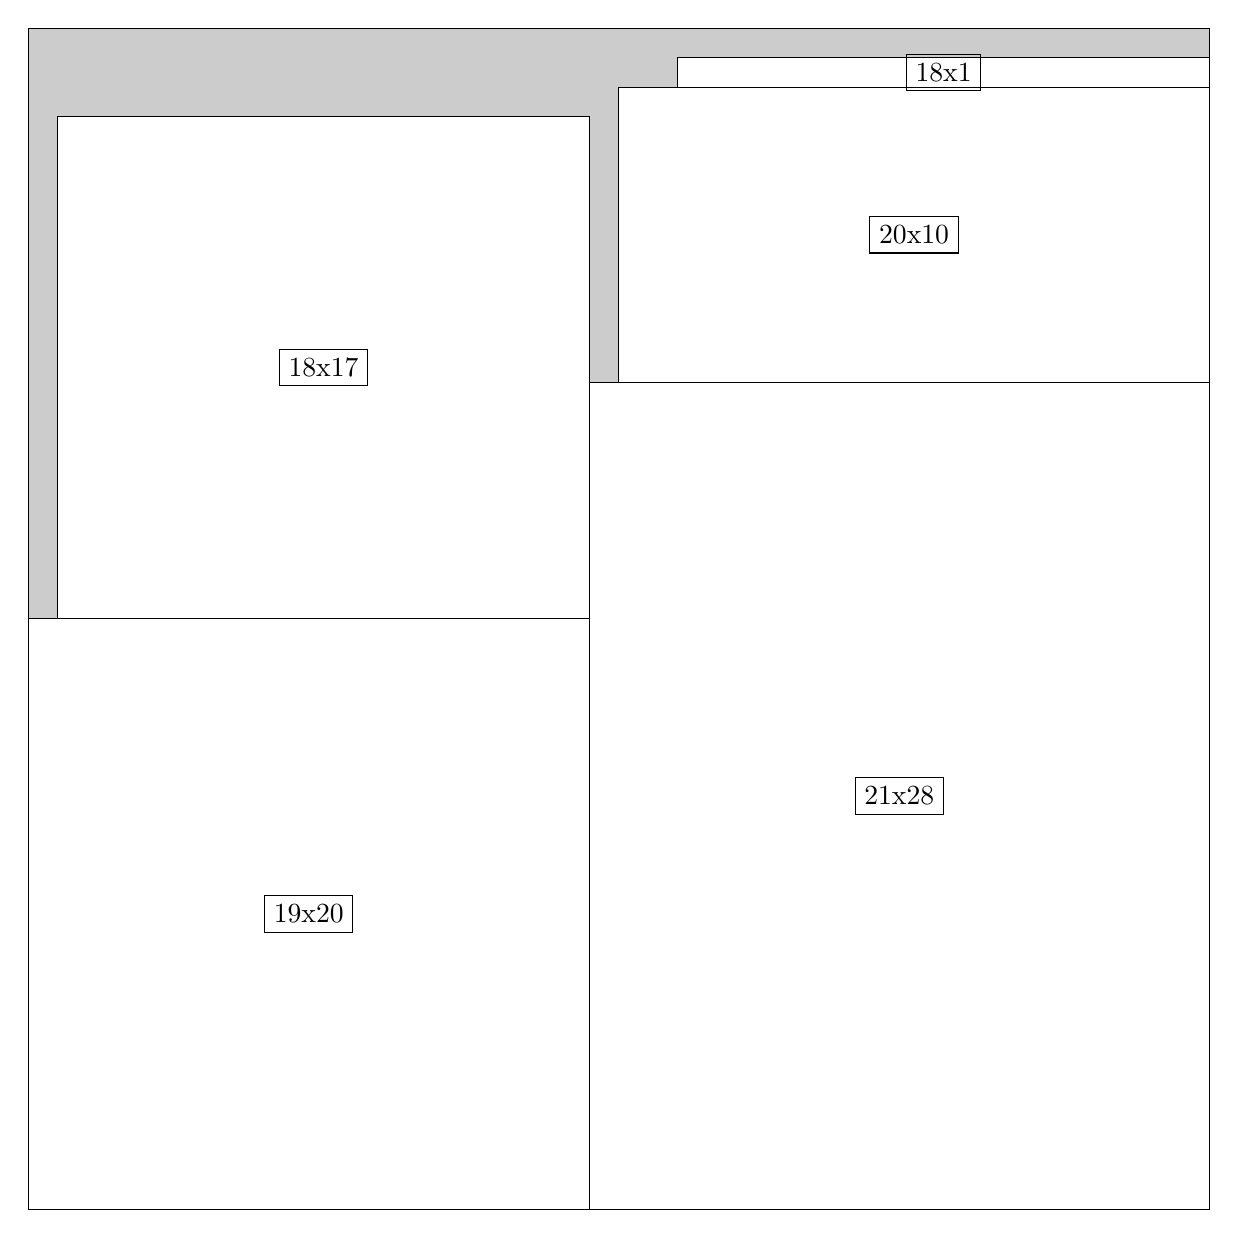
\begin{tikzpicture}[shorten >=1pt,scale=1.0,every node/.style={scale=1.0},->]
\tikzstyle{vertex}=[circle,fill=black!25,minimum size=14pt,inner sep=0pt]
\filldraw[fill=gray!40!white, draw=black] (0,0) rectangle (15.0,15.0);
\foreach \name/\x/\y/\w/\h in {21x28/7.125/0.0/7.875/10.5,20x10/7.5/10.5/7.5/3.75,18x1/8.25/14.25/6.75/0.375,19x20/0.0/0.0/7.125/7.5,18x17/0.375/7.5/6.75/6.375}
\filldraw[fill=white!40!white, draw=black] (\x,\y) rectangle node[draw] (\name) {\name} ++(\w,\h);
\end{tikzpicture}


w =21 , h =28 , x =19 , y =0 , v =588
\par
w =20 , h =10 , x =20 , y =28 , v =200
\par
w =18 , h =1 , x =22 , y =38 , v =18
\par
w =19 , h =20 , x =0 , y =0 , v =380
\par
w =18 , h =17 , x =1 , y =20 , v =306
\par
\newpage


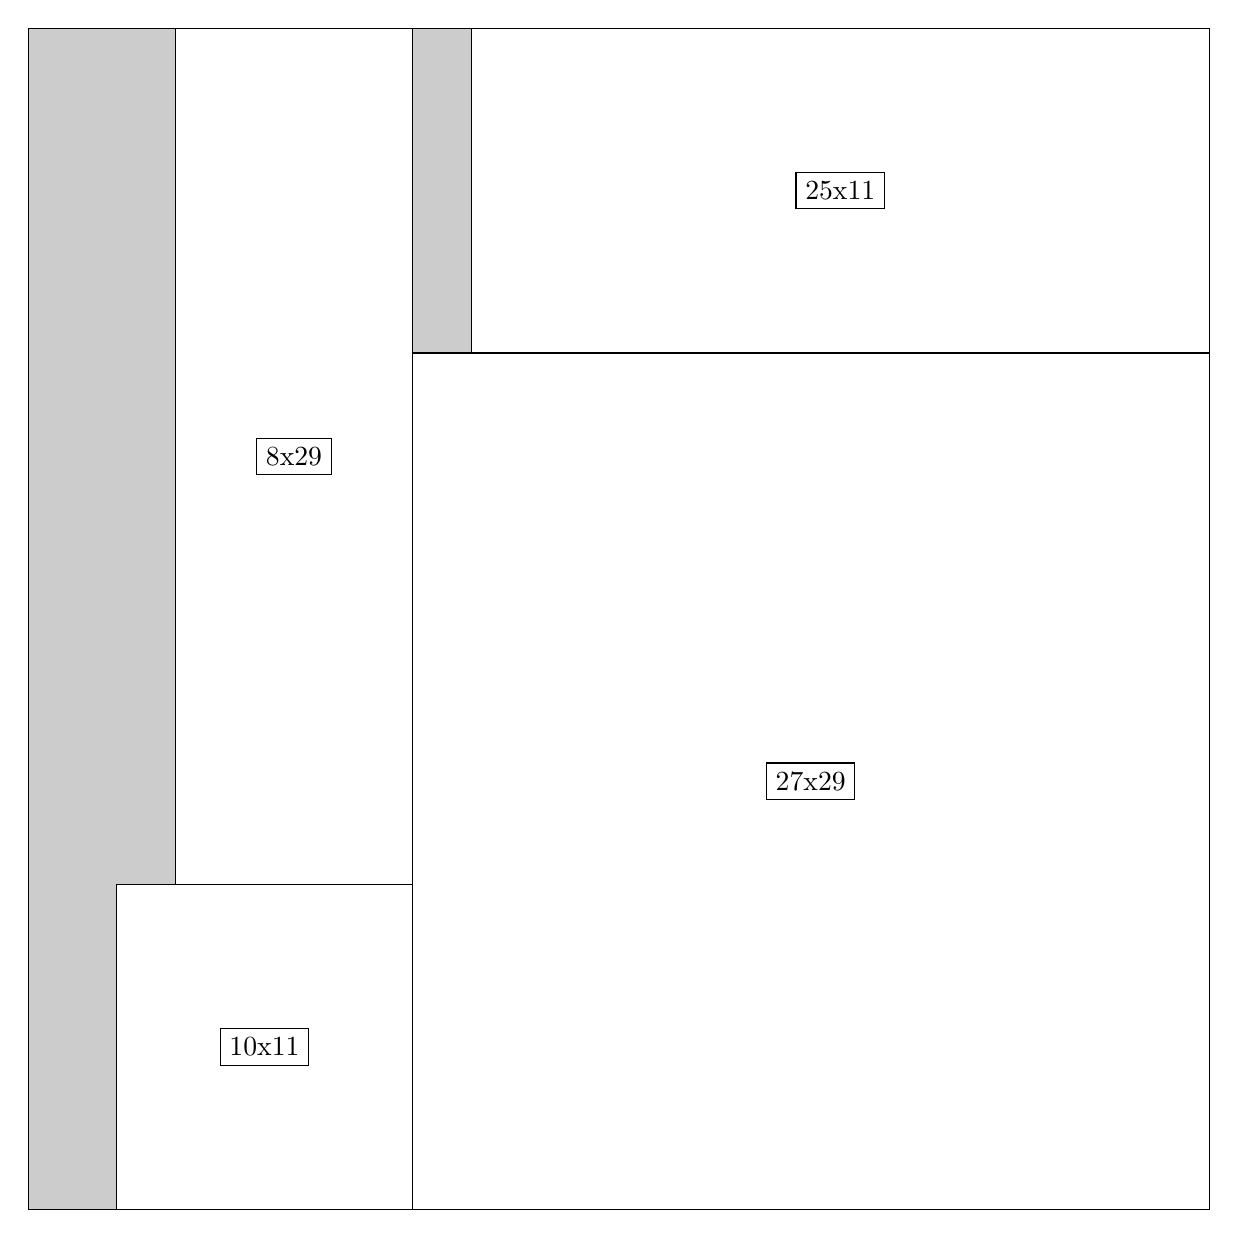
\begin{tikzpicture}[shorten >=1pt,scale=1.0,every node/.style={scale=1.0},->]
\tikzstyle{vertex}=[circle,fill=black!25,minimum size=14pt,inner sep=0pt]
\filldraw[fill=gray!40!white, draw=black] (0,0) rectangle (15.0,15.0);
\foreach \name/\x/\y/\w/\h in {27x29/4.875/0.0/10.125/10.875,25x11/5.625/10.875/9.375/4.125,10x11/1.125/0.0/3.75/4.125,8x29/1.875/4.125/3.0/10.875}
\filldraw[fill=white!40!white, draw=black] (\x,\y) rectangle node[draw] (\name) {\name} ++(\w,\h);
\end{tikzpicture}


w =27 , h =29 , x =13 , y =0 , v =783
\par
w =25 , h =11 , x =15 , y =29 , v =275
\par
w =10 , h =11 , x =3 , y =0 , v =110
\par
w =8 , h =29 , x =5 , y =11 , v =232
\par
\newpage


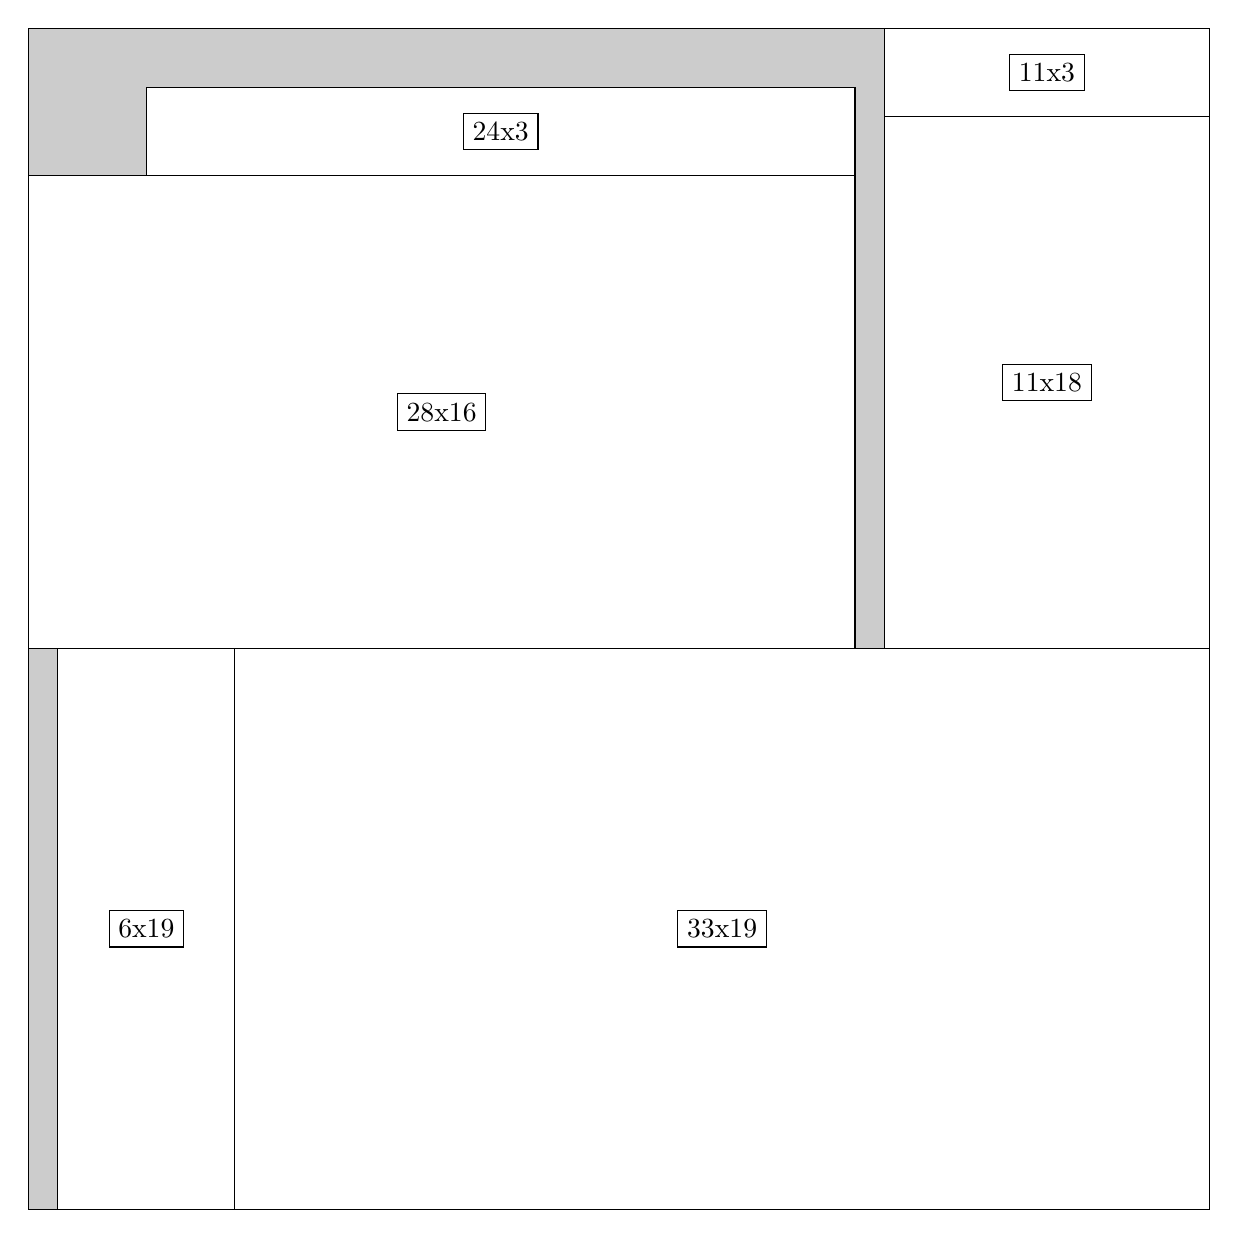
\begin{tikzpicture}[shorten >=1pt,scale=1.0,every node/.style={scale=1.0},->]
\tikzstyle{vertex}=[circle,fill=black!25,minimum size=14pt,inner sep=0pt]
\filldraw[fill=gray!40!white, draw=black] (0,0) rectangle (15.0,15.0);
\foreach \name/\x/\y/\w/\h in {33x19/2.625/0.0/12.375/7.125,6x19/0.375/0.0/2.25/7.125,11x18/10.875/7.125/4.125/6.75,11x3/10.875/13.875/4.125/1.125,28x16/0.0/7.125/10.5/6.0,24x3/1.5/13.125/9.0/1.125}
\filldraw[fill=white!40!white, draw=black] (\x,\y) rectangle node[draw] (\name) {\name} ++(\w,\h);
\end{tikzpicture}


w =33 , h =19 , x =7 , y =0 , v =627
\par
w =6 , h =19 , x =1 , y =0 , v =114
\par
w =11 , h =18 , x =29 , y =19 , v =198
\par
w =11 , h =3 , x =29 , y =37 , v =33
\par
w =28 , h =16 , x =0 , y =19 , v =448
\par
w =24 , h =3 , x =4 , y =35 , v =72
\par
\newpage


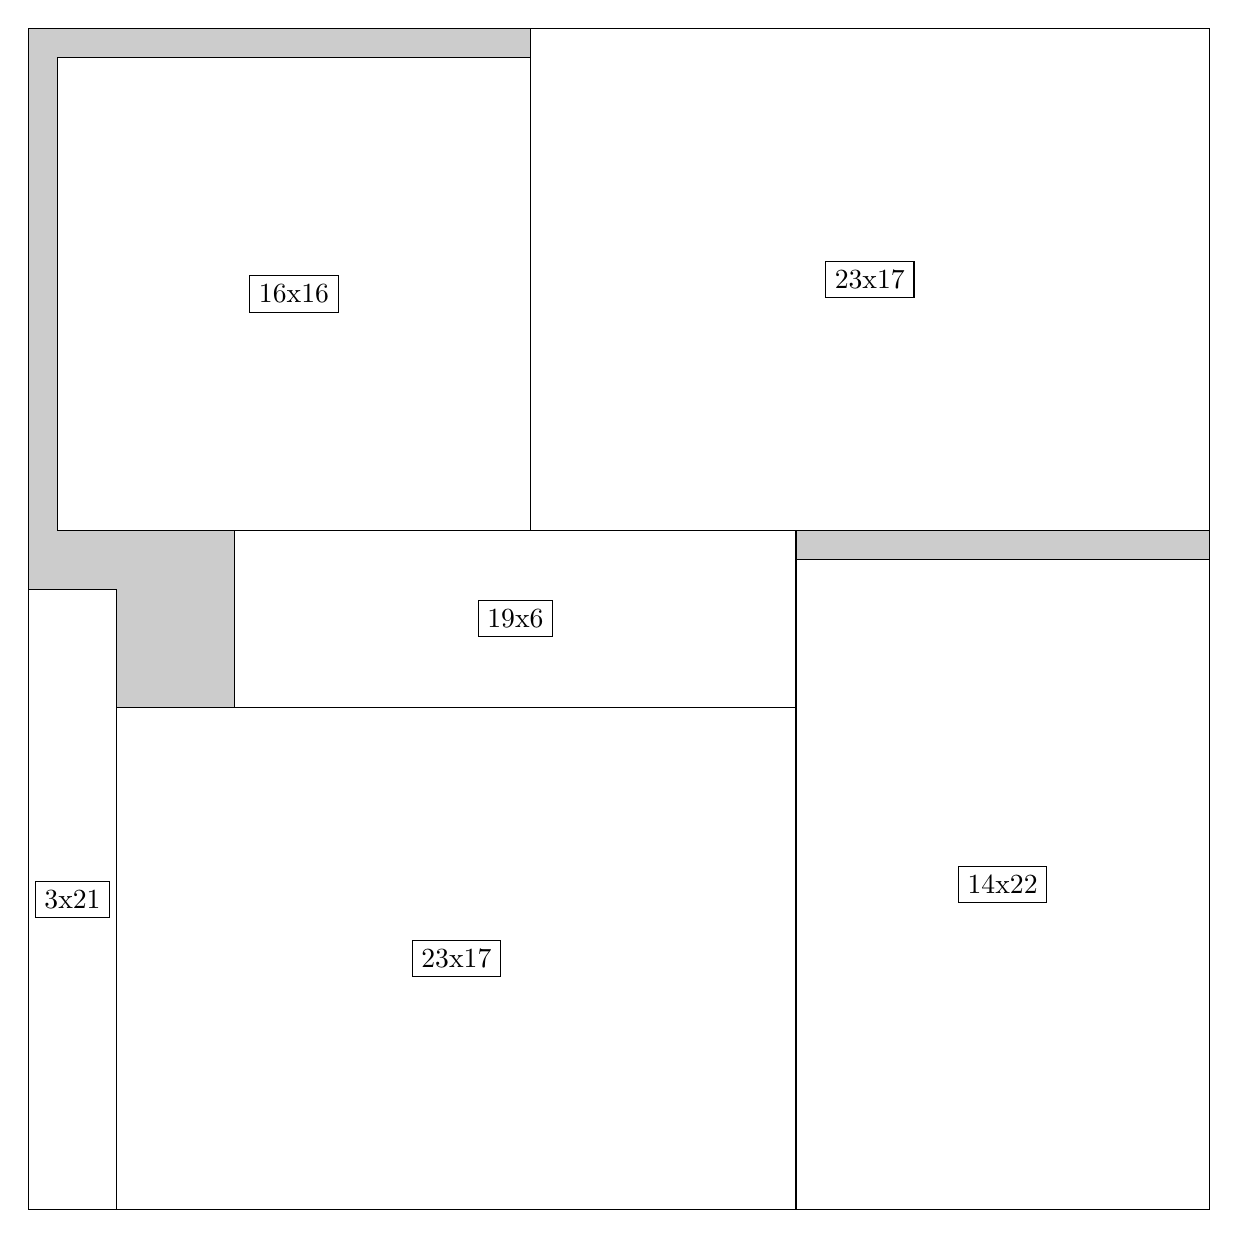
\begin{tikzpicture}[shorten >=1pt,scale=1.0,every node/.style={scale=1.0},->]
\tikzstyle{vertex}=[circle,fill=black!25,minimum size=14pt,inner sep=0pt]
\filldraw[fill=gray!40!white, draw=black] (0,0) rectangle (15.0,15.0);
\foreach \name/\x/\y/\w/\h in {14x22/9.75/0.0/5.25/8.25,23x17/1.125/0.0/8.625/6.375,19x6/2.625/6.375/7.125/2.25,3x21/0.0/0.0/1.125/7.875,23x17/6.375/8.625/8.625/6.375,16x16/0.375/8.625/6.0/6.0}
\filldraw[fill=white!40!white, draw=black] (\x,\y) rectangle node[draw] (\name) {\name} ++(\w,\h);
\end{tikzpicture}


w =14 , h =22 , x =26 , y =0 , v =308
\par
w =23 , h =17 , x =3 , y =0 , v =391
\par
w =19 , h =6 , x =7 , y =17 , v =114
\par
w =3 , h =21 , x =0 , y =0 , v =63
\par
w =23 , h =17 , x =17 , y =23 , v =391
\par
w =16 , h =16 , x =1 , y =23 , v =256
\par
\newpage


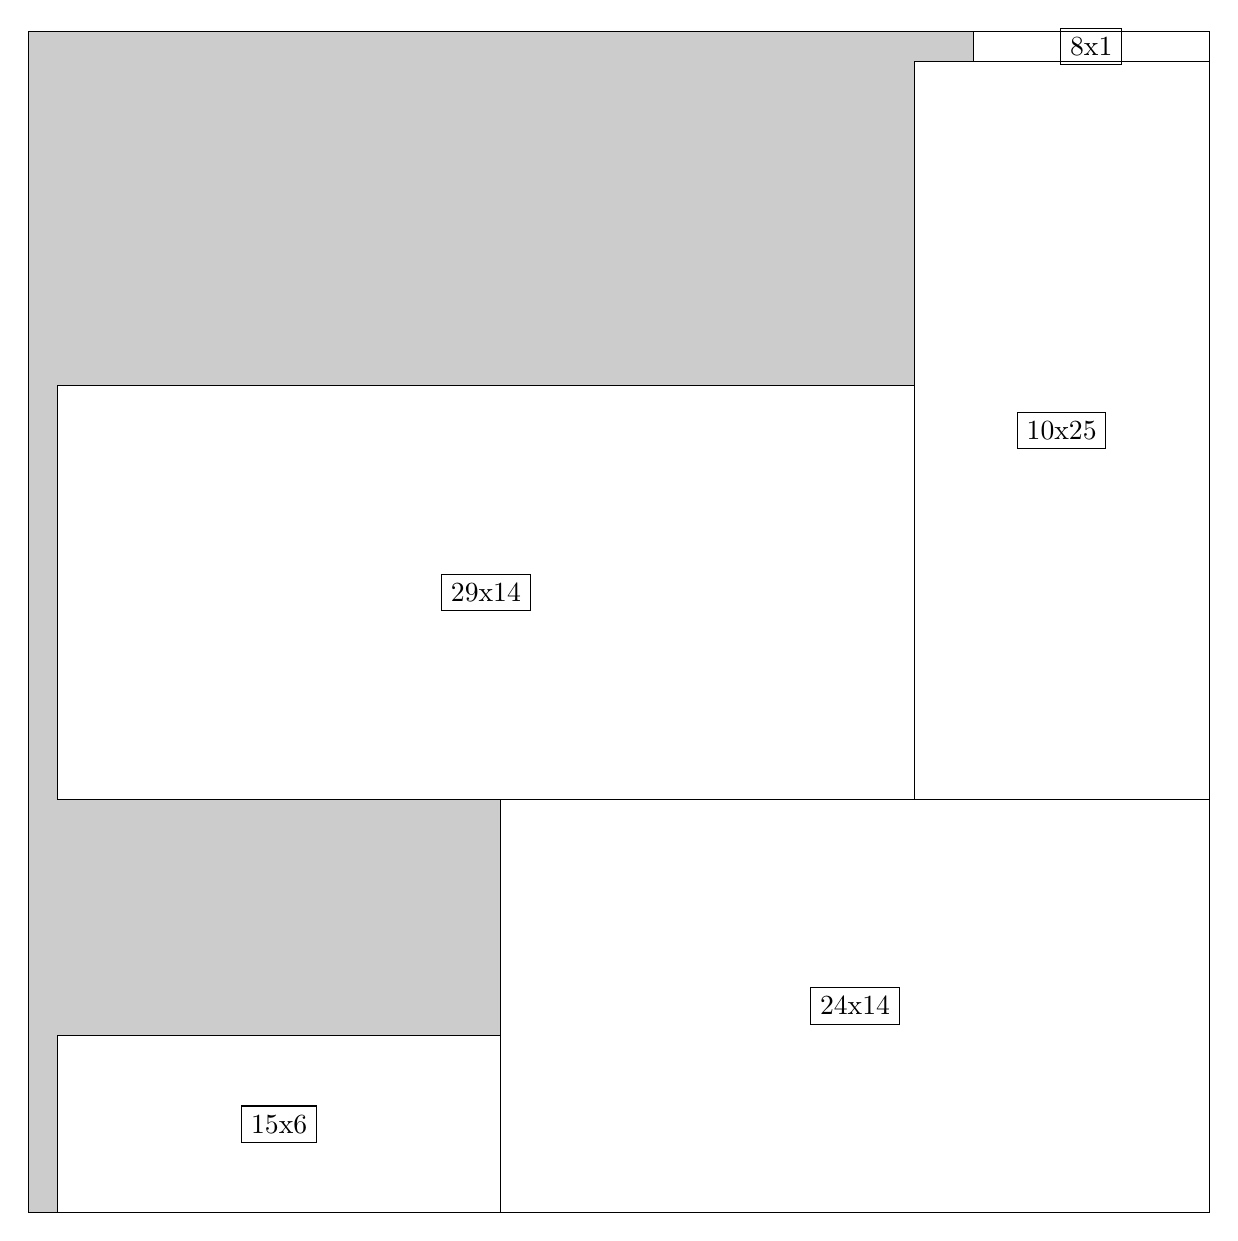
\begin{tikzpicture}[shorten >=1pt,scale=1.0,every node/.style={scale=1.0},->]
\tikzstyle{vertex}=[circle,fill=black!25,minimum size=14pt,inner sep=0pt]
\filldraw[fill=gray!40!white, draw=black] (0,0) rectangle (15.0,15.0);
\foreach \name/\x/\y/\w/\h in {24x14/6.0/0.0/9.0/5.25,15x6/0.375/0.0/5.625/2.25,10x25/11.25/5.25/3.75/9.375,8x1/12.0/14.625/3.0/0.375,29x14/0.375/5.25/10.875/5.25}
\filldraw[fill=white!40!white, draw=black] (\x,\y) rectangle node[draw] (\name) {\name} ++(\w,\h);
\end{tikzpicture}


w =24 , h =14 , x =16 , y =0 , v =336
\par
w =15 , h =6 , x =1 , y =0 , v =90
\par
w =10 , h =25 , x =30 , y =14 , v =250
\par
w =8 , h =1 , x =32 , y =39 , v =8
\par
w =29 , h =14 , x =1 , y =14 , v =406
\par
\newpage


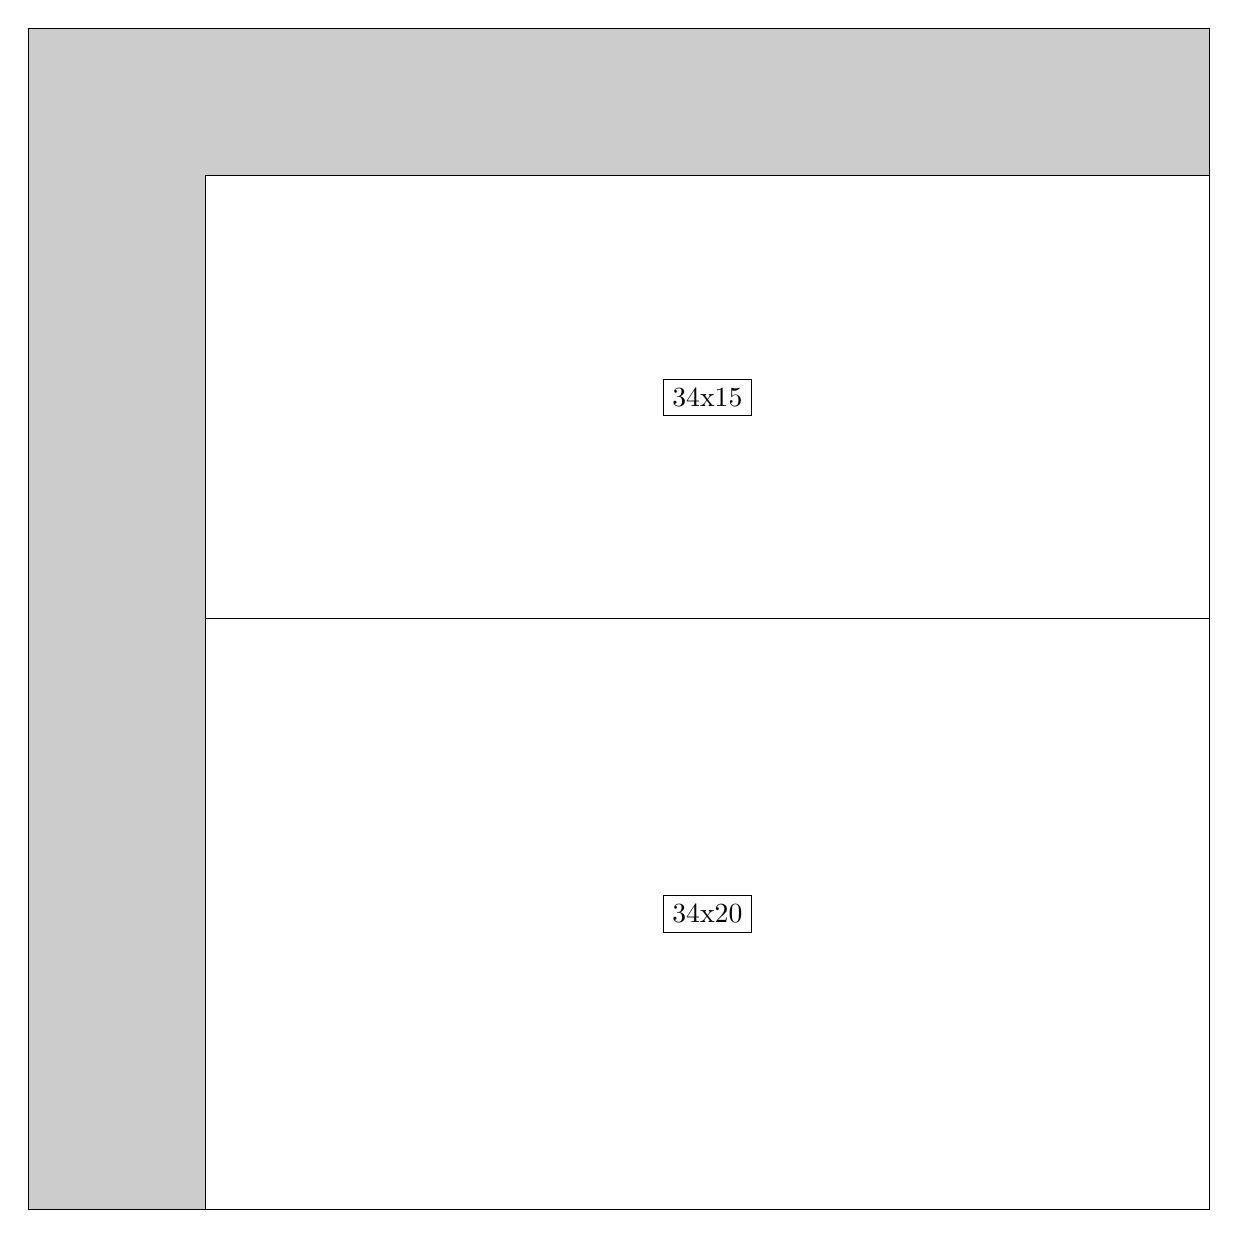
\begin{tikzpicture}[shorten >=1pt,scale=1.0,every node/.style={scale=1.0},->]
\tikzstyle{vertex}=[circle,fill=black!25,minimum size=14pt,inner sep=0pt]
\filldraw[fill=gray!40!white, draw=black] (0,0) rectangle (15.0,15.0);
\foreach \name/\x/\y/\w/\h in {34x20/2.25/0.0/12.75/7.5,34x15/2.25/7.5/12.75/5.625}
\filldraw[fill=white!40!white, draw=black] (\x,\y) rectangle node[draw] (\name) {\name} ++(\w,\h);
\end{tikzpicture}


w =34 , h =20 , x =6 , y =0 , v =680
\par
w =34 , h =15 , x =6 , y =20 , v =510
\par
\newpage


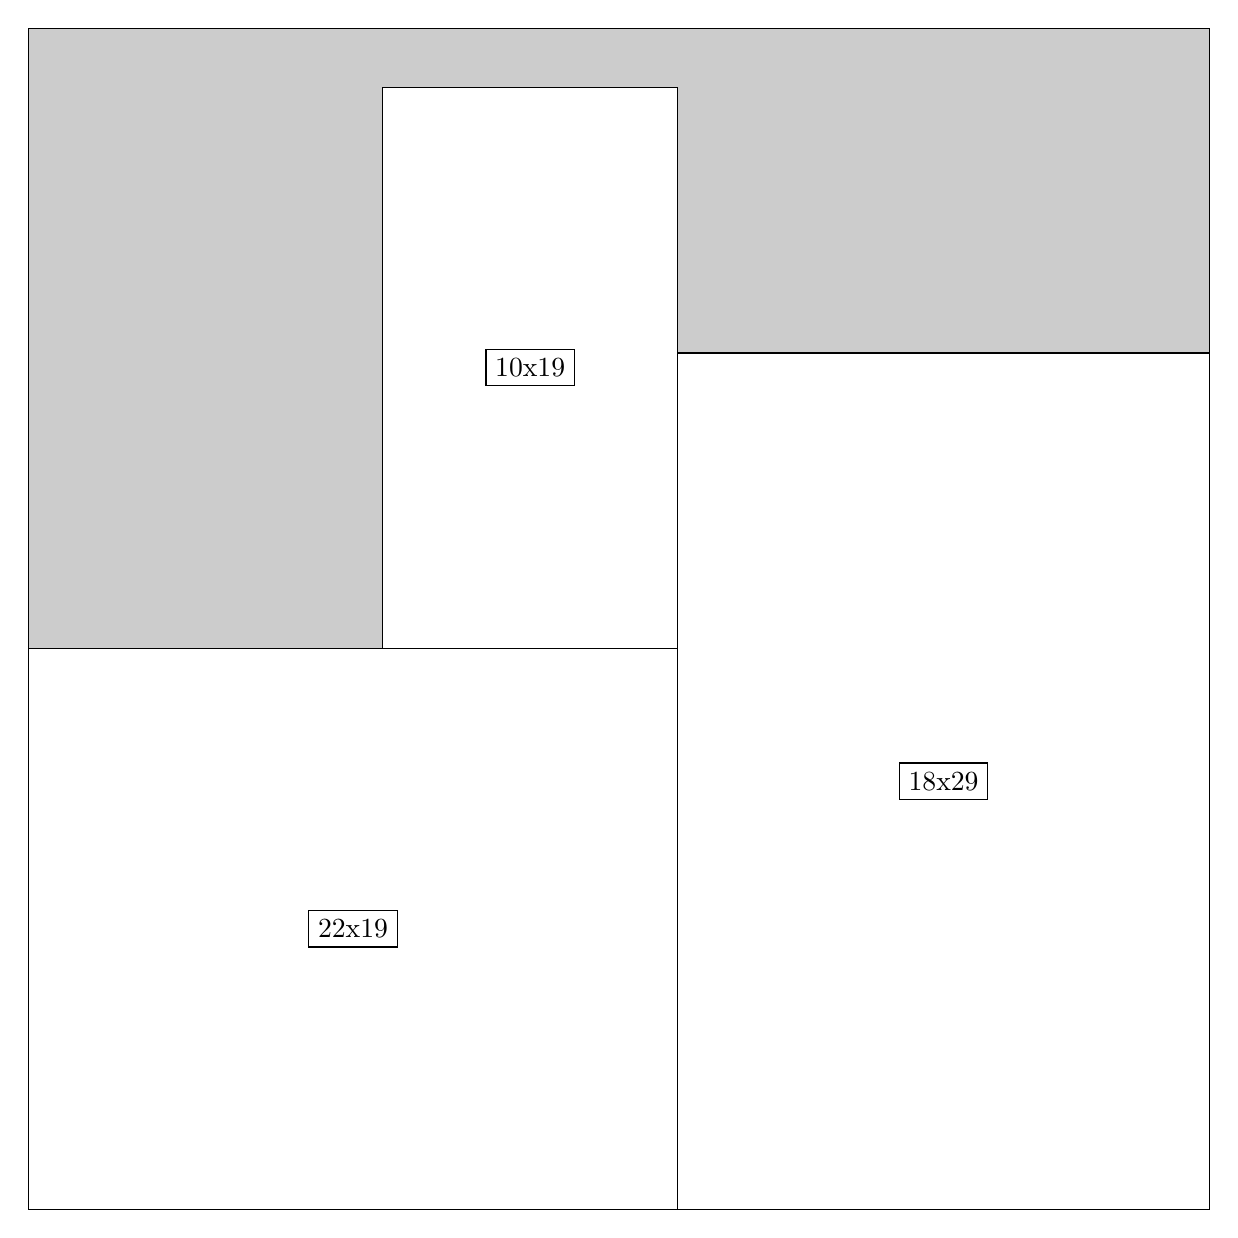
\begin{tikzpicture}[shorten >=1pt,scale=1.0,every node/.style={scale=1.0},->]
\tikzstyle{vertex}=[circle,fill=black!25,minimum size=14pt,inner sep=0pt]
\filldraw[fill=gray!40!white, draw=black] (0,0) rectangle (15.0,15.0);
\foreach \name/\x/\y/\w/\h in {18x29/8.25/0.0/6.75/10.875,22x19/0.0/0.0/8.25/7.125,10x19/4.5/7.125/3.75/7.125}
\filldraw[fill=white!40!white, draw=black] (\x,\y) rectangle node[draw] (\name) {\name} ++(\w,\h);
\end{tikzpicture}


w =18 , h =29 , x =22 , y =0 , v =522
\par
w =22 , h =19 , x =0 , y =0 , v =418
\par
w =10 , h =19 , x =12 , y =19 , v =190
\par
\newpage


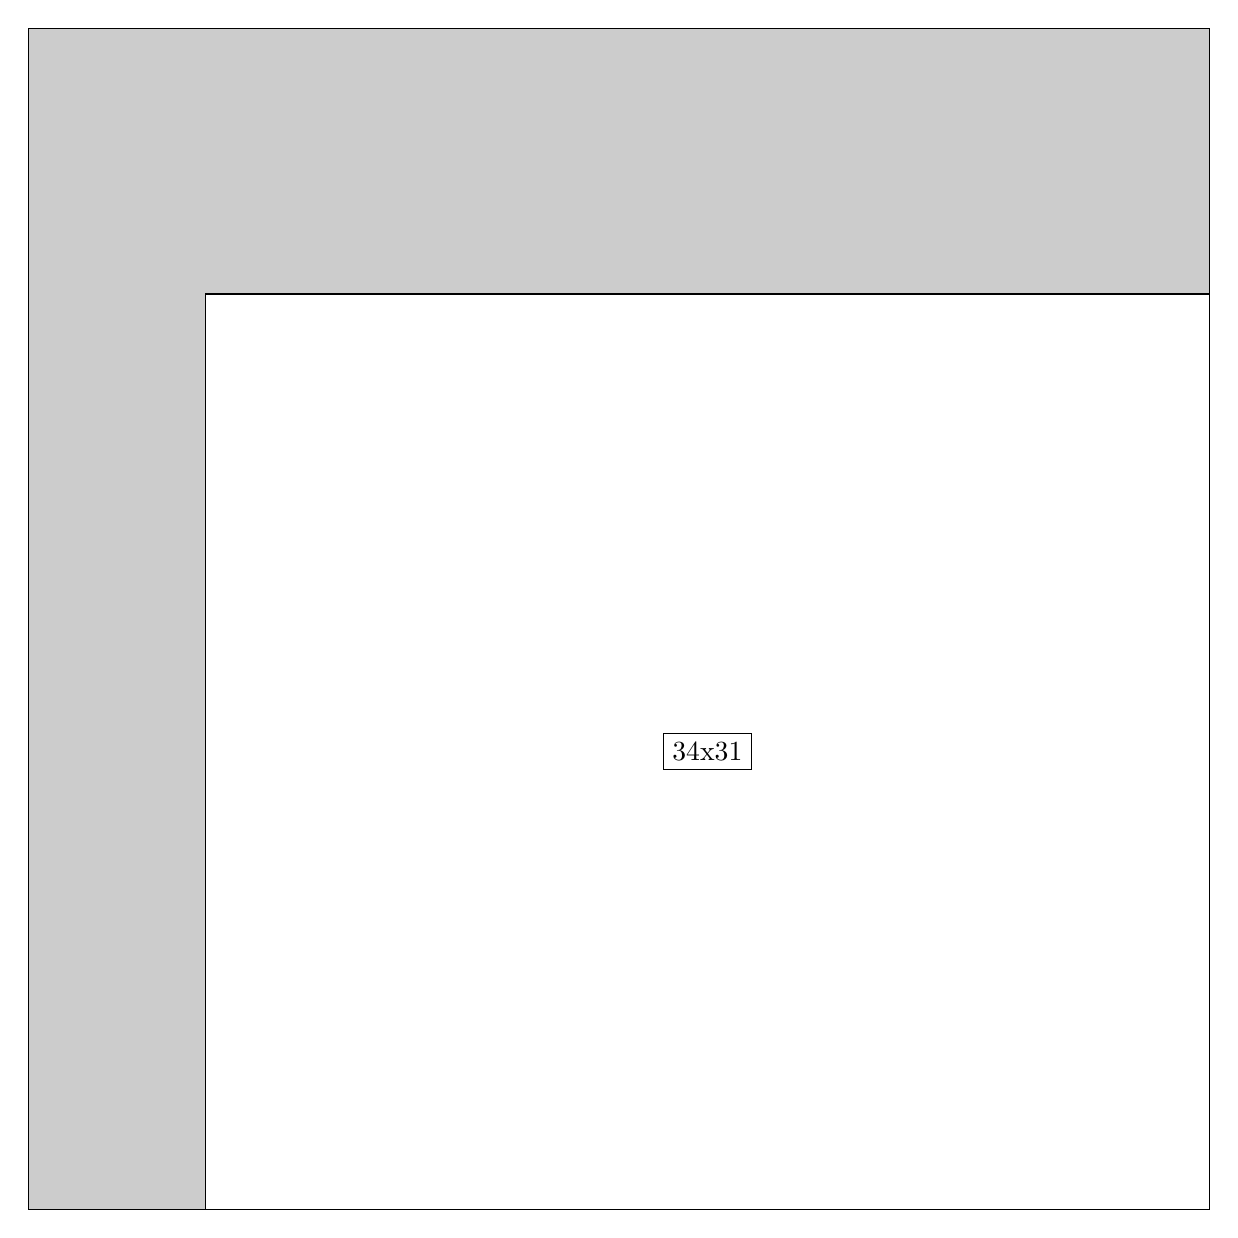
\begin{tikzpicture}[shorten >=1pt,scale=1.0,every node/.style={scale=1.0},->]
\tikzstyle{vertex}=[circle,fill=black!25,minimum size=14pt,inner sep=0pt]
\filldraw[fill=gray!40!white, draw=black] (0,0) rectangle (15.0,15.0);
\foreach \name/\x/\y/\w/\h in {34x31/2.25/0.0/12.75/11.625}
\filldraw[fill=white!40!white, draw=black] (\x,\y) rectangle node[draw] (\name) {\name} ++(\w,\h);
\end{tikzpicture}


w =34 , h =31 , x =6 , y =0 , v =1054
\par
\newpage


\end{document}